% Canonical publication manuscript. tools/build_publication.py synchronizes the Markdown.
\documentclass[11pt,a4paper]{article}
\usepackage{fontspec}
\setmainfont{texgyrepagella-regular.otf}[BoldFont=texgyrepagella-bold.otf,ItalicFont=texgyrepagella-italic.otf,BoldItalicFont=texgyrepagella-bolditalic.otf]
\setsansfont{Arial}
\setmonofont[Scale=0.85]{Consolas}
\usepackage{amsmath,amssymb,graphicx,booktabs,longtable,array}
\usepackage{unicode-math}
\setmathfont{texgyrepagella-math.otf}
\usepackage[margin=25mm]{geometry}
\usepackage{xcolor,hyperref,caption,pdflscape}
\newcommand{\FloatBarrier}{\clearpage}
\newenvironment{proof}{\par\noindent\textit{Proof.}\ }{\hfill$\square$\par}
\hypersetup{colorlinks=true,linkcolor=blue!45!black,citecolor=blue!45!black,urlcolor=blue!45!black,pdftitle={SRG Attractor Dynamics: Selective Retention and Certified Convergence under Returning Drive},pdfauthor={Hilmir Frímann Halldórsson},bookmarksnumbered=true}
\captionsetup{font=small,labelfont=bf}
\newtheorem{theorem}{Theorem}[section]
\newtheorem{proposition}[theorem]{Proposition}
\newtheorem{corollary}[theorem]{Corollary}
\numberwithin{equation}{section}
\setlength{\parskip}{4pt}
\setlength{\parindent}{0pt}
\setlength{\emergencystretch}{2em}
\clubpenalty=10000\widowpenalty=10000\displaywidowpenalty=10000
\raggedbottom
\newcommand{\R}{\mathbb R}
\newcommand{\Cset}{\mathcal C}
\newcommand{\atanTwo}{\operatorname{atan2}}
\newcommand{\diag}{\operatorname{diag}}
\title{SRG Attractor Dynamics:\\Selective Retention and Certified\\Convergence under Returning Drive}
\author{Hilmir Frímann Halldórsson}
\date{21 October 2026\\[6pt]\large v0.1 --- Publication edition}
\renewcommand{\maketitle}{\begin{center}
{\LARGE SRG Attractor Dynamics:\par}
\vspace{4mm}{\Large Selective Retention and Certified\par Convergence under Returning Drive\par}
\vspace{7mm}Hilmir Frímann Halldórsson\par
\vspace{4mm}21 October 2026\par
\vspace{4mm}\textbf{v0.1 --- Publication edition}\par
\end{center}\vspace{4mm}}
\begin{document}
\maketitle
\begin{abstract}
A plotted point can move because a measurement changes, because a state evolves, or because a numerical selection changes at a tie. These possibilities have different implications for an attractor. We examine the procedures printed with Figures 3 and 4 of the historical note \emph{SGR: simulation steps} and synthesize four accepted analyses of their dynamics. Figure 3's plotted centroid is a statistic of a newly evaluated field, not a carried particle. In its exactly symmetric, nonempty-mask setting, that centroid is fixed at the origin. Figure 4 instead carries a three-component state through a clipped, driven Euler increment and a nonlinear remapping. Without drive, the remapping attracts to a circle while leaving azimuth neutral. Under an advancing, exponentially fading drive, each admissible trajectory converges to a point on that circle. The endpoint can retain angular traces of initial size and tilt, transferred by the drive before remapping removes their direct representation. Analytic first-order comparisons distinguish these two channels of retention; saved finite calculations illustrate them. Returning the drive changes the asymptotic question. Three saved return blocks contract selected angular differences without erasing them exactly. A separate exact-real computer-assisted certificate proves that the complete 800-update return map has a unique attracting fixed point within specified two-dimensional regions at exactly $\alpha=1/32$. Five indexed saved states, interpreted as exact dyadic inputs, enter the certified region and subsequently converge under indefinite repetition. These conclusions concern the stated recurrence and domains. The geometric framework is a passive analytical reference, and no physical confinement, global attraction, or thermodynamic consequence is inferred. All scientific computations reported here are inherited; paper preparation performed no scientific reruns.
\end{abstract}
\clearpage
\section*{Plain-language overview}
\addcontentsline{toc}{section}{Plain-language overview}
The main result is a change in what survives when the input changes. A fading input allows different starting states to settle at different angular positions. Repeating the input can instead pull a specified collection of states toward the same repeating response. The second conclusion is proved locally for one exact coupling strength, with a separate proof that five saved states reach the region where it applies.

Three distinctions make this result intelligible. First, a measurement marker is not necessarily an evolving object. The marker associated with historical Figure 3 summarizes a field evaluated on a grid; the rule does not carry that marker into the next update. Its near-central position therefore does not demonstrate physical attraction. Second, the remapping in historical Figure 4 is an active part of a recurrence. It removes positive-ray scale and contracts a meridional coordinate, while preserving an angular coordinate when the drive is absent. Third, information can change its representation before one of these removals occurs. The driven increment can turn a starting-size or starting-tilt difference into an angular difference. Removing size or tilt afterward does not undo that angular trace.

When the same 800-update input block returns, the state continues from where the preceding block left it. In the saved finite experiments, nearby angular traces get smaller over three blocks but remain different. That observation alone cannot justify an infinite-time claim. The accepted certificate supplies the missing argument: on explicit two-coordinate regions, the exact block map sends the region into itself and shrinks distances in a specified norm. This establishes one repeating response there and convergence toward it. The five entry results apply to the exact real numbers represented by the saved floating-point states; they do not retrospectively certify the unknown exact histories that generated those files.

The Tri-Octagon and crystal framework helps distinguish reference coordinates, views and native dynamical quantities. It supplies no force or wall. The circle and toroidal surface discussed below arise from the printed remapping itself. The paper keeps that active operation separate from a passive geometric measurement view throughout.
\tableofcontents
\clearpage

\section{Question, sources and evidential scope}\label{sec:scope}
\subsection{From a central marker to a repeating response}
The term ``attractor'' is meaningful only after specifying a state, its evolution law, the time convention and a notion of approach. Our starting point is the historical note \emph{SGR: simulation steps}, dated 1 August 2025, especially its Figures 3 and 4 and the accompanying text on physical pages 5--8 \cite{historical}. We retain the title's SGR spelling when identifying that source and use SRG for the present research programme. The question is mathematical: what does the printed procedure actually evolve, what does the displayed point measure, and in what sense do states approach a common object?

Four accepted investigations supply the evidence. CA01 establishes source provenance and the distinction between a field statistic and a carried state. CA02 studies which initial-state information can reach the limiting angular position under fading drive. CA03 continues saved checkpoints under advancing and returning schedules and derives a small-coupling block-response theorem. CA04 supplies an exact-strength, exact-real certificate for a complete returning block, followed by a separately scoped entry test \cite{ca01,ca02,ca03,ca04}. The presentation below connects these results into one argument; it does not assume that a historical drawing determines the dynamics.

The supplied scientific reviews accepted the respective analyses without required corrections within their stated scopes \cite{review01,review02,review03,review04}. These are documented internal scientific reviews, not a claim of journal peer review. Their reports and independent-review evidence archives accompany this edition. The original historical producer and all of its run inputs have not been recovered. In particular, the missing original coupling, initial state, complete producer code and numerical environment prevent an exact reconstruction of the historical Figure 4 trajectory. The bounded later calculations use declared diagnostic parameters; these are not recovered historical inputs.

\subsection{Three kinds of result}
An analytic result follows from the stated recurrence and hypotheses. A finite numerical observation describes saved calculations, with their finite duration and arithmetic. A computer-assisted certificate combines mathematical inequalities with outward enclosures for the exact-real map. These categories support different claims. A small floating-point residual is useful for locating a candidate but proves neither existence nor attraction. A finite contraction ratio establishes neither exact erasure nor indefinite convergence. Conversely, a rigorous contraction proof on a region says more than numerical convergence from a single starting point, but less than global attraction.

The certificate's scope is deliberately narrow: exact $\alpha=1/32$, the complete 800-update returning schedule, the specified two-coordinate domains, and the five exact saved inputs for the entry extension. Its proof arithmetic and review history are described in Section~\ref{sec:certificate}. The paper inherits that certificate; neither it nor any scientific checker was executed during manuscript preparation. Hash checks, table transcription, figure copying, typesetting and visual inspection are editorial operations. The supplementary claim ledger records the source and status of each main assertion, equation family, table and figure.

\subsection{What the geometry means}
We distinguish three uses of geometry. The historical remapping is an active update of the state. Intrinsic coordinates describe the surface produced by that update. The accepted Tri-Octagon/crystal reference is a separate, passive analytical instrument. Only the first changes the recurrence. Neither the intrinsic chart nor the reference mesh is an additional physical ball, crystal, container or confining force. This distinction is necessary even when a plot makes the resulting motion look bounded.

\section{The carried state and the measurement marker}\label{sec:model}
\subsection{A complete recurrence, with an advancing clock}
In historical Figure 4, the carried state is $s_n=(x_n,y_n,z_n)\in\R^3$. Set $\rho=(x^2+y^2)^{1/2}$ and $L=\|s\|$. The cyclic roll is $Cs=(z,x,y)$. The prescribed four-term drive, called the REFU curve in the source, is
\begin{equation}\label{eq:drive}
H(t)=2e^{-t/2}\cos t+e^{-3t/10}\sin t+\frac32e^{-7t/10}+e^{-2t/5}.
\end{equation}
No additional state variable stores or accumulates this function. Write
\begin{equation}\label{eq:torque}
A(s)=s\times Cs=(y^2-xz,\ z^2-xy,\ x^2-yz).
\end{equation}
For the clock value $t_n$, the complete update is
\begin{equation}\label{eq:update}
\begin{aligned}
q_n&=\alpha H(t_n)A(s_n),\\
\widehat q_n&=q_n\min\left(1,\frac{4/5}{\|q_n\|+1/100000}\right),\\
u_n&=s_n+\frac1{10}\widehat q_n,\qquad s_{n+1}=P(u_n).
\end{aligned}
\end{equation}
The clipping factor, its small denominator offset, the Euler step and the remapping are all retained. Velocity is not carried separately. The drive is a scalar prescribed by the clock, whereas the torque direction depends on the current state. For fading drive, $t_n=n/10$ in the exact-real formulation. Floating-point source implementations evaluate their corresponding clock expression in machine arithmetic; the certificate later treats rational times exactly.

For an incoming nonzero, off-axis vector, let $\varphi=\atanTwo(y,x)$ and $\vartheta=\atanTwo(\rho,z)$. The historical TGMO remapping, with major radius one and minor radius one half, is
\begin{equation}\label{eq:remap}
P(s)=\left(\left(1+\frac{z}{2L}\right)\frac{x}{\rho},\ 
\left(1+\frac{z}{2L}\right)\frac{y}{\rho},\ \frac{\rho}{2L}\right).
\end{equation}
This is equivalent to its trigonometric form with output radius $1+\tfrac12\cos\vartheta$ and output height $\tfrac12\sin\vartheta$. At the axis, azimuth is undefined: there is no unique smooth extension of this formula there. A numerical convention at a singular input is not an analytic resolution of that singularity. Statements below require an admissible first remap; subsequent domain bounds are supplied explicitly.

\begin{table}[htbp]
\centering\small
\caption{Notation and distinctions used throughout the paper.}\label{tab:notation}
\begin{tabular}{p{.18\textwidth}p{.74\textwidth}}
\toprule
Symbol & Meaning \\
\midrule
$s,u,q,\widehat q$ & Carried state, pre-remap state, raw and clipped increments. \\
$C,\Cset$ & Cyclic roll operator and limiting circle, respectively. \\
$\rho,L$ & Cylindrical radius and Euclidean norm. \\
$\varphi,\vartheta,\theta$ & Azimuth, incoming polar angle, and torus meridional coordinate. \\
$P,K$ & Active remapping and the closed upper half-torus containing its image. \\
$\Phi_{\alpha,k},E_{\alpha,k}$ & Lifted limiting phase and vector endpoint for starting clock index $k$. \\
$T_\alpha,N$ & Returning block map and block length $N=800$. \\
$c,v$ & Certificate coordinates $c=\cos\theta$, $v=\tan(\varphi/2)$. \\
$X,B$ & Small root region and larger contraction/entry region. \\
\bottomrule
\end{tabular}
\end{table}

The source calls TGMO the Toroidal Geometric Memory Operator and RPCO the Recursive Phase Compression Operator. These labels do not make the two historical figures identical procedures. Their printed clipping and measurement rules differ. Equations~\eqref{eq:drive}--\eqref{eq:remap} specify the Figure 4 recurrence being analysed; source terminology is not substituted for its operations.

\subsection{Why Figure 3's point need not be an attractor}
Historical Figure 3 instead evaluates a vector field on a fixed $100\times100$ grid in $[-5,5]^2$. Its components share the scalar factor $H(t)/(1+X^2+Y^2)$, with direction obtained by rotating the local tangential direction through the prescribed offset $0.05\sin(0.1t)$. Here $H(t)$ denotes the Figure 3 amplitude curve with its printed symbolic coefficients; no equality of its historical parameters with those in equation \eqref{eq:drive} is asserted. The printed exact magnitude before clipping is therefore
\begin{equation}\label{eq:field}
M(X,Y,t)=\frac{|H(t)|}{1+X^2+Y^2},\qquad M_{\rm clip}=\min(M,1).
\end{equation}
The small time-dependent change of direction cancels from the magnitude. The plotted point is the centroid of grid positions whose magnitude is strictly below the fifth percentile. The field is recomputed; that point is not the initial condition for the next time step. This is a changing measurement of a prescribed field, not a particle recurrence.

\begin{proposition}[Exact centroid symmetry]\label{thm:centroid}
On an inversion-paired grid, with exact radial magnitudes and the printed strict percentile rule, every selected point is accompanied by its negative. If the mask is nonempty, its centroid is the origin. If it is empty, its centroid is undefined.
\end{proposition}
\begin{proof}
The magnitudes at $(X,Y)$ and $(-X,-Y)$ are equal. A single strict threshold consequently either selects both or selects neither. Pair sums vanish. Dividing the sum by the selected count is valid only for a positive count.
\end{proof}

For nonzero $H$, small magnitudes occur toward the outer grid, including its corners. A central centroid need not itself belong to that selected region; the even-sized grid need not contain the origin at all. At $H=0$ every magnitude is equal and the strict mask is empty. On this square, $|H|\ge51$ makes the exactly clipped magnitudes uniformly one, again yielding an empty strict mask. Percentile ties can also change the selected count away from a nominal five percent.

Saved CA01 tests show why a tiny moving centroid can nevertheless appear. At $H=4.5$, one ordinary binary64 grid evaluation selected 498 sites and gave centroid $(0.0148067,0)$; a binary32 evaluation selected 500 and gave $(-0.0339394,0)$. A deliberately paired radial evaluation selected 496 and balanced to numerical zero. In a fully clipped $H=100$ diagnostic, roundoff in the computed magnitudes straddled one, producing 120 selected sites and a spurious nonempty centroid. These are observations about tie sensitivity, not reconstructions of the original image \cite{ca01}.

A surviving related script uses the first flattened argmin and an epsilon-adjusted clipping expression rather than the printed centroid rule. Its existence helps explain another possible selection mechanism, but does not identify it as the missing historical producer. The source distinction must remain unresolved. Figure~\ref{fig:mask} illustrates the measurement mechanism without turning a grid statistic into a dynamical state.

\begin{landscape}
\begin{figure}[p]
\centering
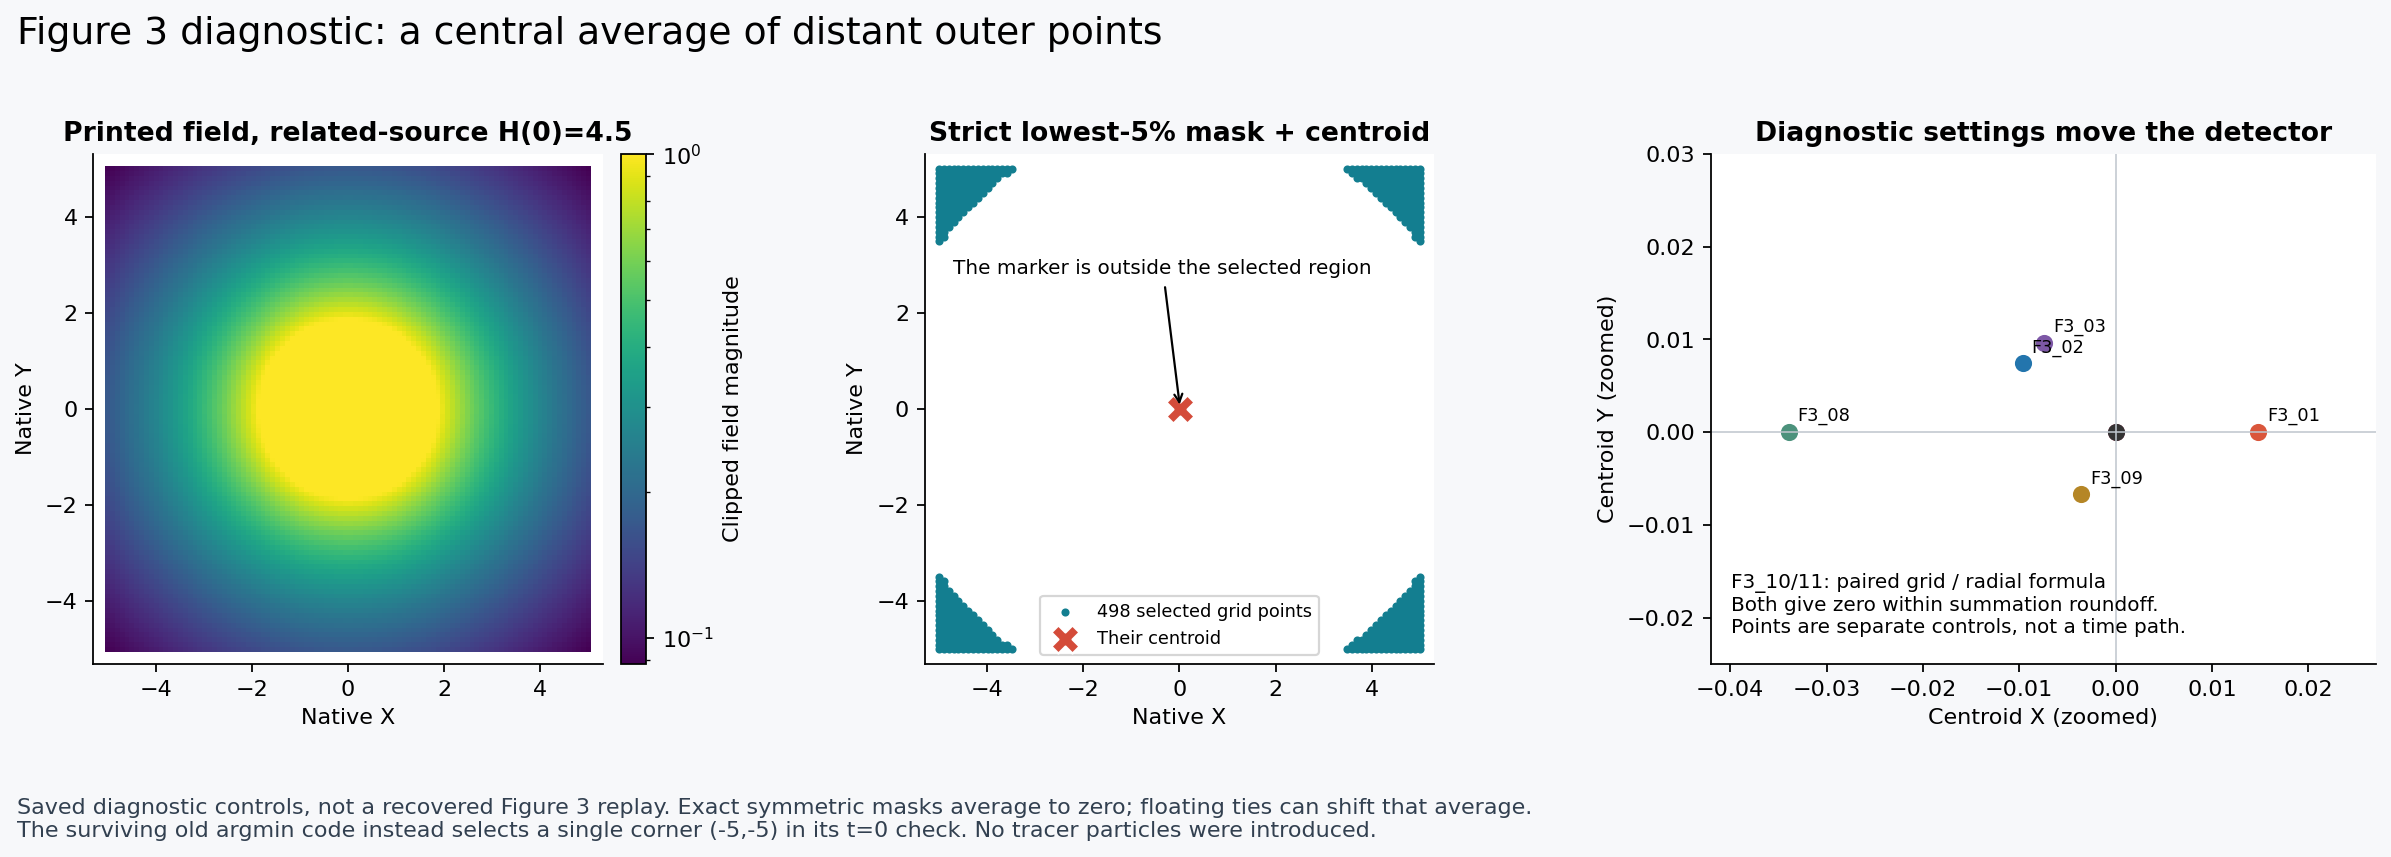
\includegraphics[width=\linewidth,height=0.80\textheight,keepaspectratio]{figures/01_mask.png}
\caption{Field measurement and centroid selection. Reused unchanged from CA01, \texttt{plots/01\_F3\_mask\_and\_centroid.png}. This is an explanatory diagnostic, not a reproduction of historical Figure 3. Outer low-magnitude sites can have a central centroid; floating-point selection at percentile ties can change the marker. The exact nonempty-mask symmetry statement is Proposition~\ref{thm:centroid}.}\label{fig:mask}
\end{figure}
\end{landscape}

\section{What the remapping erases, and what fading drive retains}\label{sec:fading}
\subsection{A circle that attracts as a set}
The Figure 4 remapping has a concrete geometric effect independent of its historical name. It is homogeneous of degree zero for positive scale:
\begin{equation}\label{eq:scale}
P(\lambda s)=P(s)\qquad(\lambda>0).
\end{equation}
It is not an idempotent projection. For example, $P(1,0,0)=(1,0,1/2)$ whereas $P^2(1,0,0)=(1+1/(2\sqrt5),0,1/\sqrt5)$. Repeated remapping continues to change a meridional coordinate.

The image lies in the upper half of the torus whose closure is
\begin{equation}\label{eq:torus}
K=\{s:(\rho-1)^2+z^2=1/4,\ z\ge0,\ \rho\ge1/2\}.
\end{equation}
This surface is a consequence of the active formula, not a fitted physical boundary. Parametrize it by
\begin{equation}\label{eq:torusparam}
s(\theta,\varphi)=((1+\tfrac12\cos\theta)\cos\varphi,
(1+\tfrac12\cos\theta)\sin\varphi,\tfrac12\sin\theta),\quad 0\le\theta\le\pi.
\end{equation}
With zero drive, $\varphi$ is unchanged and the meridional map is
\begin{equation}\label{eq:g}
g(\theta)=\atanTwo(1+\tfrac12\cos\theta,\tfrac12\sin\theta),\qquad
g'(\theta)=-\frac{1/4+(1/2)\cos\theta}{5/4+\cos\theta}.
\end{equation}
It takes $[0,\pi]$ into $[\pi/3,\pi/2]$ and satisfies $|g'|\le1/3$ on $[0,\pi/2]$. Its unique fixed meridian gives
\begin{equation}\label{eq:circle}
\begin{aligned}
c_*&=\cos\theta_*=(\sqrt3-1)/2,\\
\rho_*&=(3+\sqrt3)/4,\qquad z_*=\tfrac12\sqrt{\sqrt3/2},\\
\Cset&=\{s_*(\varphi)=(\rho_*\cos\varphi,\rho_*\sin\varphi,z_*):\varphi\in\R\}.
\end{aligned}
\end{equation}
The transverse multipliers are zero for positive-ray scale and $\sqrt3-2$ for meridional perturbations; the azimuthal multiplier is one. Thus $\Cset$ attracts as a set, but an individual point of it does not attract an open set of azimuths in the unforced system. The negative meridional multiplier produces alternating approach, not a persistent period-three orbit. The contraction of $g$ rules out other meridional cycles.

The Euler increment should not be mistaken for a length-preserving rotation. Although $s\cdot\widehat q=0$, the finite step obeys
\begin{equation}\label{eq:eulernorm}
\|s+\tfrac1{10}\widehat q\|^2=\|s\|^2+\tfrac1{100}\|\widehat q\|^2.
\end{equation}
It increases squared norm whenever the increment is nonzero. A continuous perpendicular vector field would conserve norm; that fact does not apply unchanged to this finite Euler operation. Subsequent remapping has a separate, stronger effect on scale.

\begin{landscape}
\begin{figure}[p]
\centering
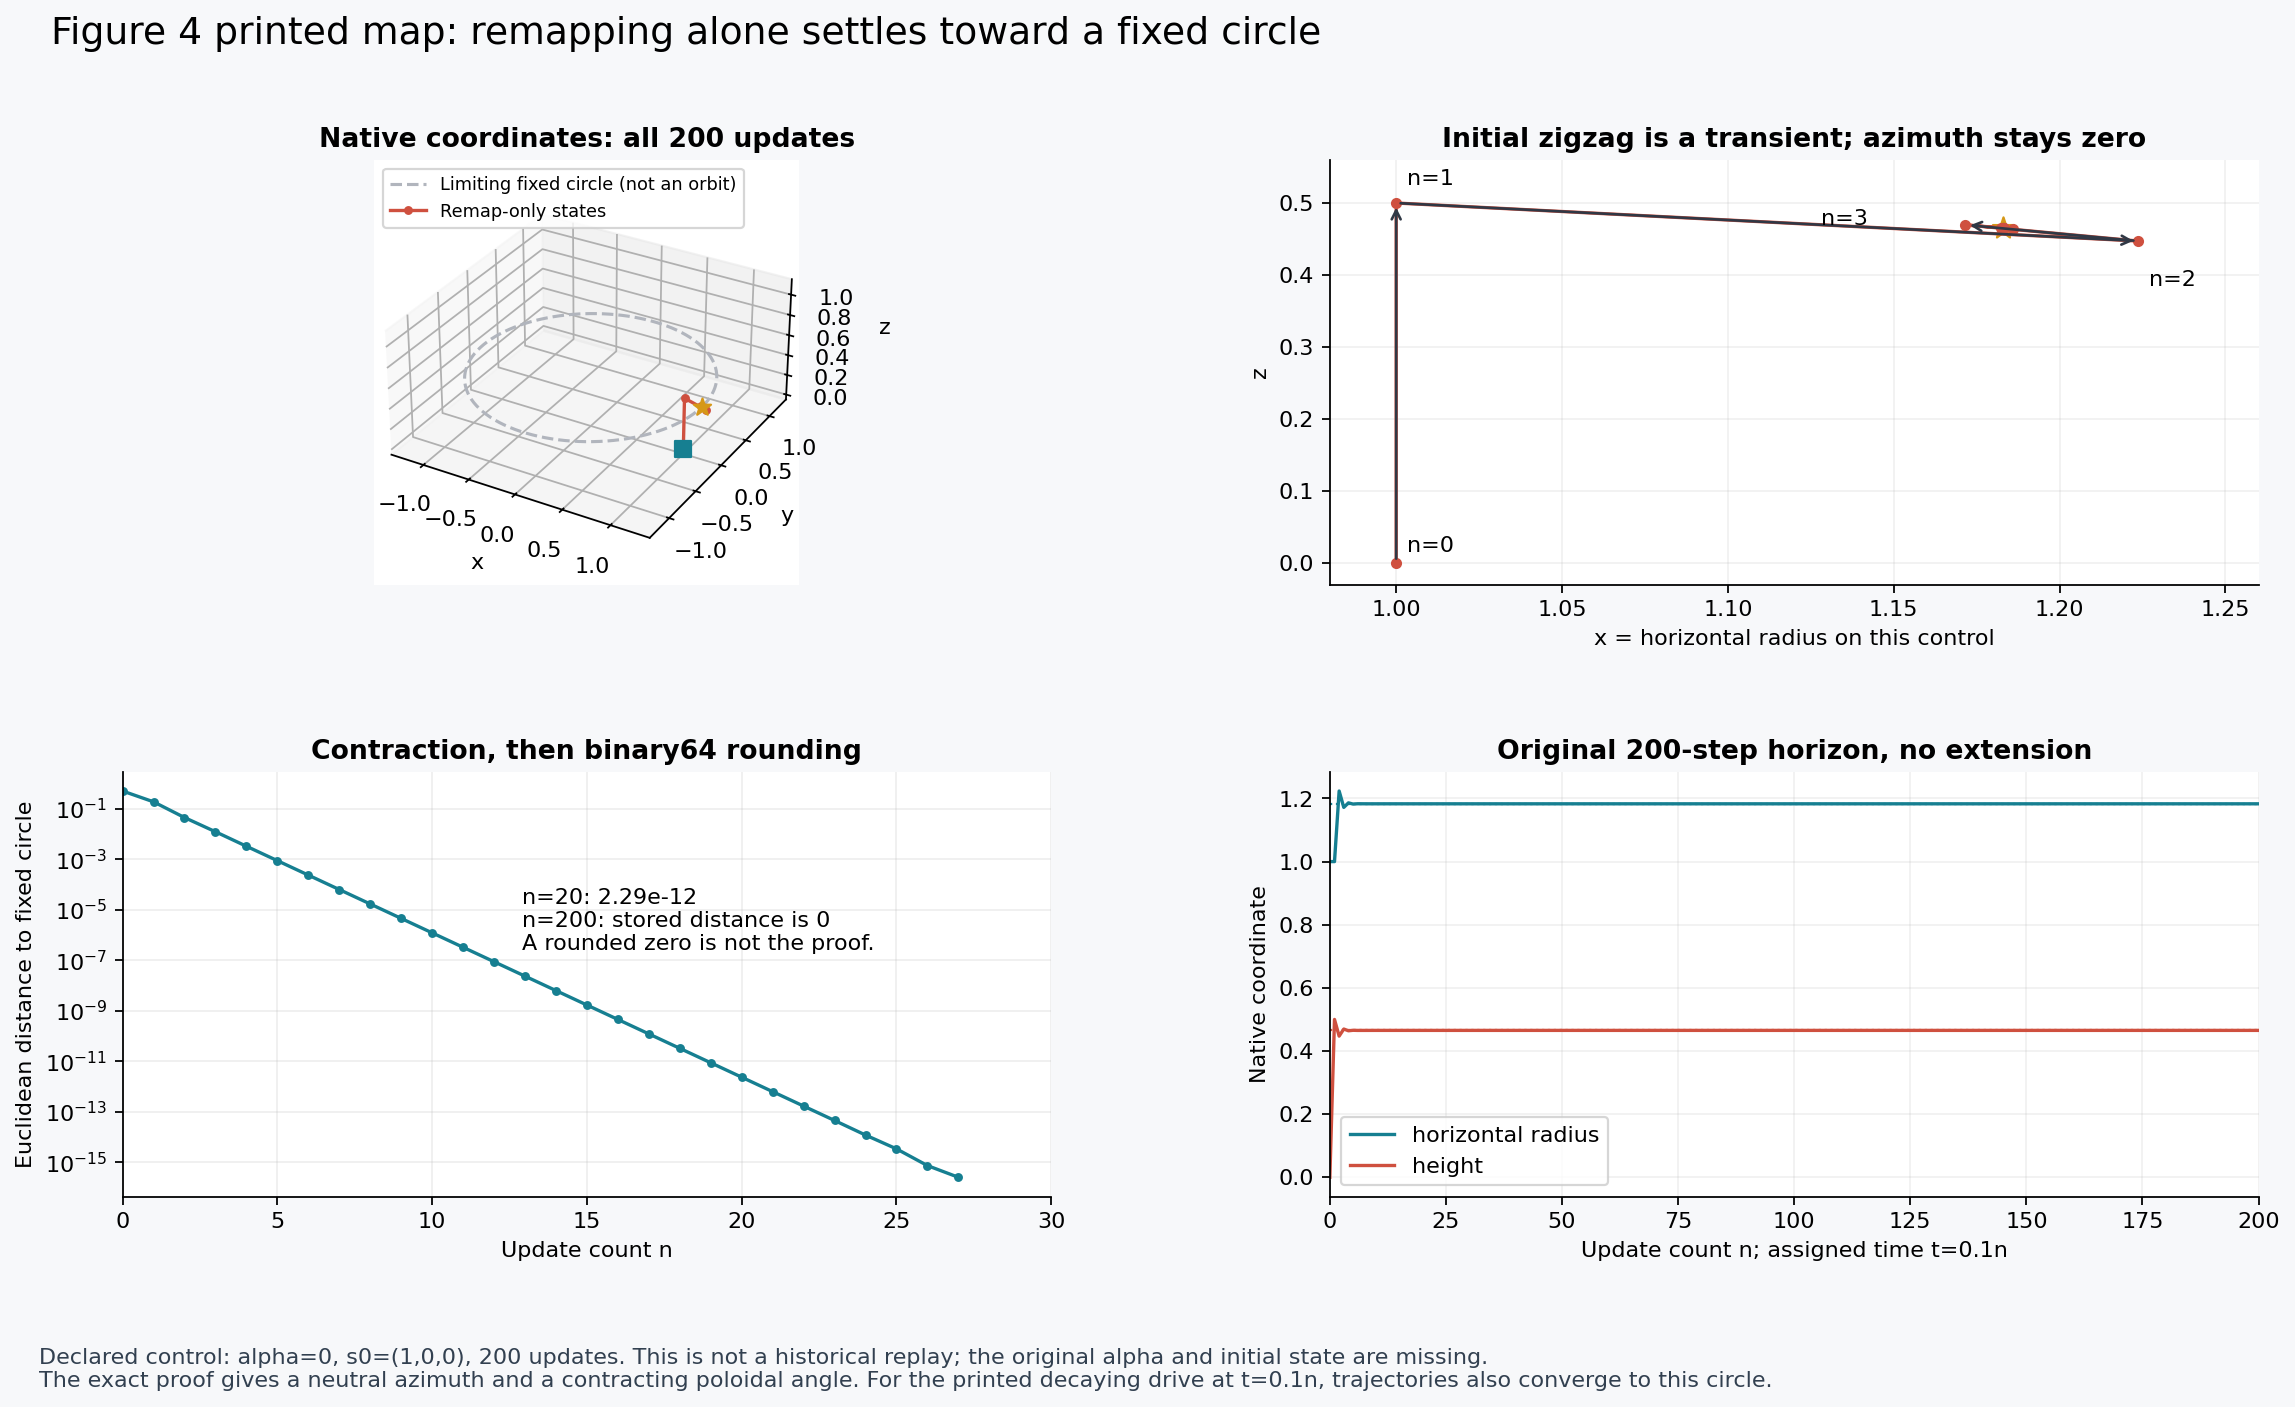
\includegraphics[width=\linewidth,height=0.80\textheight,keepaspectratio]{figures/02_remap.png}
\caption{The active remap and its limiting circle. Unchanged CA01 figure \texttt{plots/02\_F4\_remap\_only.png}, using a declared zero-drive diagnostic. Repeated remapping contracts the meridional coordinate while leaving azimuth neutral. A plotted floating-point distance reaching zero does not mean exact finite-time arrival. The toroidal surface belongs to the recurrence, not to the passive Tri-Octagon reference.}\label{fig:remap}
\end{figure}
\end{landscape}

\subsection{Convergence with an advancing, fading input}
Fading drive changes the limiting angular position but does not sustain a nonzero loop. The needed bound is summability, not a visual impression that the drive looks small. Put $e_n=\widehat q_n/10$. On $K$, $\|s\|\le3/2$ and $\|A(s)\|\le\|s\|^2\le9/4$, hence
\begin{equation}\label{eq:incrementbound}
\|e_n\|\le \min\{0.08,\ 0.225|\alpha||H(n/10)|\},\qquad
\sum_{n\ge0}|H(n/10)|<\infty.
\end{equation}
The series converges by an exponential envelope. On a segment from $s\in K$ to $s+e$, the cylindrical radius is at least $0.5-0.08=0.42$. This both avoids the axis and bounds the gradients of the relevant angular coordinates.

\begin{theorem}[Endpoint under fading drive]\label{thm:fading}
Fix finite real $\alpha$ and let the clock advance as $t_n=n/10$, without resets. If the first application of $P$ is admissible, the complete exact-real recurrence~\eqref{eq:update} converges to $s_*(\varphi_\infty)\in\Cset$ for some limiting phase. A consistent azimuthal lift has absolutely summable increments. The statement does not assign a common endpoint to all initial states.
\end{theorem}
\begin{proof}
After the first remap the state belongs to $K$. The segment radius bound above gives $|\Delta\varphi_n|\le\|e_n\|/0.42$, and the right-hand side is summable. For the meridian, the output height is at least $\tfrac12(0.42)/1.58>0.1329$. At the following pre-remap step its height remains greater than $0.0529$. Consequently the iterated meridional coordinate enters $[0,\pi/2]$ after finitely many initial operations, where
\begin{equation}\label{eq:meridionalbound}
|\theta_{n+1}-\theta_*|\le\tfrac13|\theta_n-\theta_*|+\|e_n\|/0.42.
\end{equation}
Iteration of this inequality, with $\|e_n\|\to0$, gives $\theta_n\to\theta_*$. The absolutely summable lifted angular increments give $\varphi_n\to\varphi_\infty$. Substitution in~\eqref{eq:torusparam} proves full-state convergence.
\end{proof}

The circle need not be invariant under each driven step; it is the fixed set of the limiting zero-drive map. Uniform tail control on a latitude circle gives a continuous degree-one limiting phase map, so the family of endpoints covers the circle. This excludes a universal endpoint for that family. In particular, a nonzero recurring triangle or persistent loop cannot be the asymptotic behaviour of the printed recurrence with this advancing fading input. That conclusion concerns the equation, not an identification of what generated the historical raster image.

\subsection{The clock belongs in the endpoint map}
Let $F_{\alpha,k}$ denote one complete update at clock index $k$. Define the endpoint map and a consistent local phase lift by
\begin{equation}\label{eq:endpoint}
E_{\alpha,k}(s)=s_*(\Phi_{\alpha,k}(s)\bmod 2\pi),\qquad
E_{\alpha,k}=E_{\alpha,k+1}\circ F_{\alpha,k}.
\end{equation}
The index shift is essential. Composing with $E_{\alpha,0}$ instead would reset the input. The endpoint is the result of a state together with its future clock schedule.

At zero coupling, $E_0(s)=(\rho_*x/\rho,\rho_*y/\rho,z_*)$ on the admissible off-axis domain. Its phase differential is
\begin{equation}\label{eq:zerophase}
D_s\Phi_0=(-y/\rho^2,\ x/\rho^2,\ 0).
\end{equation}
It has rank one and two-dimensional local fibres: size and meridional position are erased while azimuth remains. The next section asks how a nonzero drive can transfer some of those otherwise erased differences into the retained coordinate before remapping acts.

\section{Selective angular retention under fading drive}\label{sec:retention}
\subsection{Exact increments and first-order response}
For an admissible segment, the angular change made before remapping is
\begin{equation}\label{eq:phaseincrement}
\Delta\varphi=\atanTwo(xe_y-ye_x,\rho^2+xe_x+ye_y),\qquad
\Phi_{\alpha,0}=\varphi_0+\sum_{n\ge0}\Delta\varphi_n.
\end{equation}
When $\rho>\|e_{xy}\|$, the second argument is positive and the chosen increment lies in $(-\pi/2,\pi/2)$. Subsequent remapping preserves that newly acquired azimuth. Thus the fact that $P$ erases scale cannot by itself show that the full driven step erases its angular consequences.

The accepted first derivative at zero coupling is
\begin{equation}\label{eq:firstresponse}
\begin{aligned}
D(s_0)&=\left.\partial_\alpha\Phi_{\alpha,0}(s_0)\right|_{\alpha=0}
=\frac1{10}\sum_{n\ge0}H(n/10)W(P^ns_0),\\
W(s)&=\frac{xA_y-yA_x}{\rho^2}=\frac{xz(z+y)}{\rho^2}-y.
\end{aligned}
\end{equation}
At $\alpha=0$, the angular increment vanishes identically as a function of state, so its state derivative is zero. State variations do not contribute an extra first-order term to this sum. Uniform differentiation of the infinite endpoint limit does require justification; Appendix~\ref{app:regularity} gives the accepted argument rather than treating a finite sum as its proof.

On the limiting circle, define $b=z_*^2/\rho_*=(\sqrt3-1)/4$. Then
\begin{equation}\label{eq:G}
G(\varphi)=b\cos\varphi+z_*\sin\varphi\cos\varphi-\rho_*\sin\varphi,
\qquad D(s_*(\varphi))=\tfrac1{10}S G(\varphi),
\end{equation}
where the convergent scalar sum has the closed form
\begin{equation}\label{eq:S}
\begin{aligned}
S={}&2\Re\frac1{1-e^{-0.05+0.1i}}+
\Im\frac1{1-e^{-0.03+0.1i}}\\
&+\frac{3/2}{1-e^{-0.07}}+\frac1{1-e^{-0.04}}.
\end{aligned}
\end{equation}
The cardinal values of $G$ are $b,-\rho_*,-b,\rho_*$. The first-order response is consequently a phase-dependent deformation, not a uniform angular shift. The fixed cyclic roll selects directions; rotating only an initial state while holding that operator fixed changes the experiment.

\subsection{Starting size and starting tilt are different comparisons}
For $s_0=\lambda s_*(\varphi)$ with positive $\lambda$, all zero-drive iterates after the first remap coincide. The initial torque is quadratic in size, however, and the phase response obeys
\begin{equation}\label{eq:size}
D(\lambda s_*(\varphi))=\tfrac1{10}SG(\varphi)+0.45(\lambda-1)G(\varphi).
\end{equation}
At $\varphi=0$, $G(0)=b>0$, so the half-size, reference and three-halves-size states have distinct first derivatives. Their limiting phases are therefore distinct for all sufficiently small nonzero coupling. This is an analytic local statement in $\alpha$; it does not itself establish a numerical validity threshold at $1/32$.

For a separate tilt comparison, hold the initial Euclidean norm at $L_*=\|s_*(0)\|$ and take $s_0=L_*(\cos\beta,0,\sin\beta)$. This is not a rescaled copy of the circle state. Let $\theta_1=\pi/2-\beta$, $\theta_{n+1}=g(\theta_n)$ and
\begin{equation}\label{eq:tilt}
\begin{aligned}
W_0&=L_*\frac{\sin^2\beta}{\cos\beta},\qquad
w(\theta)=\frac{(1/4)\sin^2\theta}{1+(1/2)\cos\theta},\\
D_{\rm tilt}&=\tfrac1{10}\left[Sb+H(0)(W_0-b)+\sum_{n\ge1}H(n/10)(w(\theta_n)-b)\right].
\end{aligned}
\end{equation}
The correction reflects the successive meridional states before they converge. Since $|w'|\le5/8$ and $|\theta_n-\theta_*|\le(\pi/2)3^{-(n-1)}$, its tail is controlled geometrically. The accepted strict estimates give $D_{\rm tilt}(0)<D(s_*(0))$ and $D_{\rm tilt}(\pi/4)>D(s_*(0))$. Appendix~\ref{app:regularity} retains the sign bounds. They establish a tilt-to-phase channel independently of the size-to-phase channel.

There are exact exceptions. If $s=d(1,1,1)\ne0$, then $A(s)=0$. Positive rescalings of this state have the same first remap and identical subsequent states at the same clock, even though torque at later states can become nonzero. More generally, a zero first-order coefficient or a zero first angular increment does not prove exact erasure. The scaled full step contains both the quadratic torque and its scale-dependent clipping factor; it cannot be replaced by $P(\lambda s)=P(s)$ alone.

For sufficiently small coupling on a compact admissible neighbourhood, the endpoint phase remains smooth with nonzero state gradient. Its local fibres are still two-dimensional. On the initial circle, $\partial_\varphi\Phi=1+O(\alpha)>0$, giving an invertible degree-one phase map for sufficiently small $\alpha$. Neither fact makes the full three-dimensional initial state recoverable from one limiting angle. ``Retention'' here means a nonzero response to a specified change of initial condition, not complete storage of that condition.

\subsection{What the saved finite observations add}
The CA02 calculations comprise 16 declared trajectories of 800 updates each. Their prefixes are retained as saved evidence, not rerun for this paper. Table~\ref{tab:retention} reports the relevant $\alpha=1/32$ states and inherited derivative estimates. The two comparison families remain separate. Figure~\ref{fig:retention} shows the corresponding saved diagnostic presentation.

\begin{table}[htbp]
\centering\small
\caption{Fading-drive retention: inherited CA02 values. Angles are radians at saved index 800, not certified exact endpoints. The derivatives are accepted scalar-series estimates.}\label{tab:retention}
\begin{tabular}{lrrr}
\toprule
Initial comparison & $D$ estimate & Phase at 800 & Difference from reference \\
\midrule
Reference $s_*(0)$ & 1.2054125880 & 0.034913238851 & 0 \\
Half-size & 1.1642347301 & 0.033801059304 & $-0.001112179547$ \\
Three-halves-size & 1.2465904460 & 0.036032627511 & $+0.001119388660$ \\
Equal-norm tilt $\beta=0$ & 1.1456671347 & 0.033301883984 & $-0.001611354867$ \\
Equal-norm tilt $\beta=\pi/4$ & 1.4963456589 & 0.042901847724 & $+0.007988608873$ \\
\bottomrule
\end{tabular}
\end{table}

A useful analytic remainder bound for the exact trajectory after index $N$ is
\begin{equation}\label{eq:tail}
\begin{aligned}
B_N(\alpha)=\frac{0.225|\alpha|}{0.42}\bigg[
&\frac{2e^{-0.05N}}{1-e^{-0.05}}+\frac{e^{-0.03N}}{1-e^{-0.03}}\\
&+\frac{1.5e^{-0.07N}}{1-e^{-0.07}}+\frac{e^{-0.04N}}{1-e^{-0.04}}\bigg].
\end{aligned}
\end{equation}
The saved evaluation gives $B_{800}(1/32)\simeq2.13896\times10^{-11}$. This bounds the remaining angular tail of an exact trajectory, not accumulated floating-point error in an 800-step computation. It must not be interpreted as an end-to-end error certificate for Table~\ref{tab:retention}. Saved central differences at steps $1/32$ and $1/64$ exhibit error ratios near four, consistent with the proved smooth expansion, but do not constitute a numerical third-derivative bound. The exact small-coupling distinctions and the finite nonzero differences have complementary, explicitly different statuses.

\begin{landscape}
\begin{figure}[p]
\centering
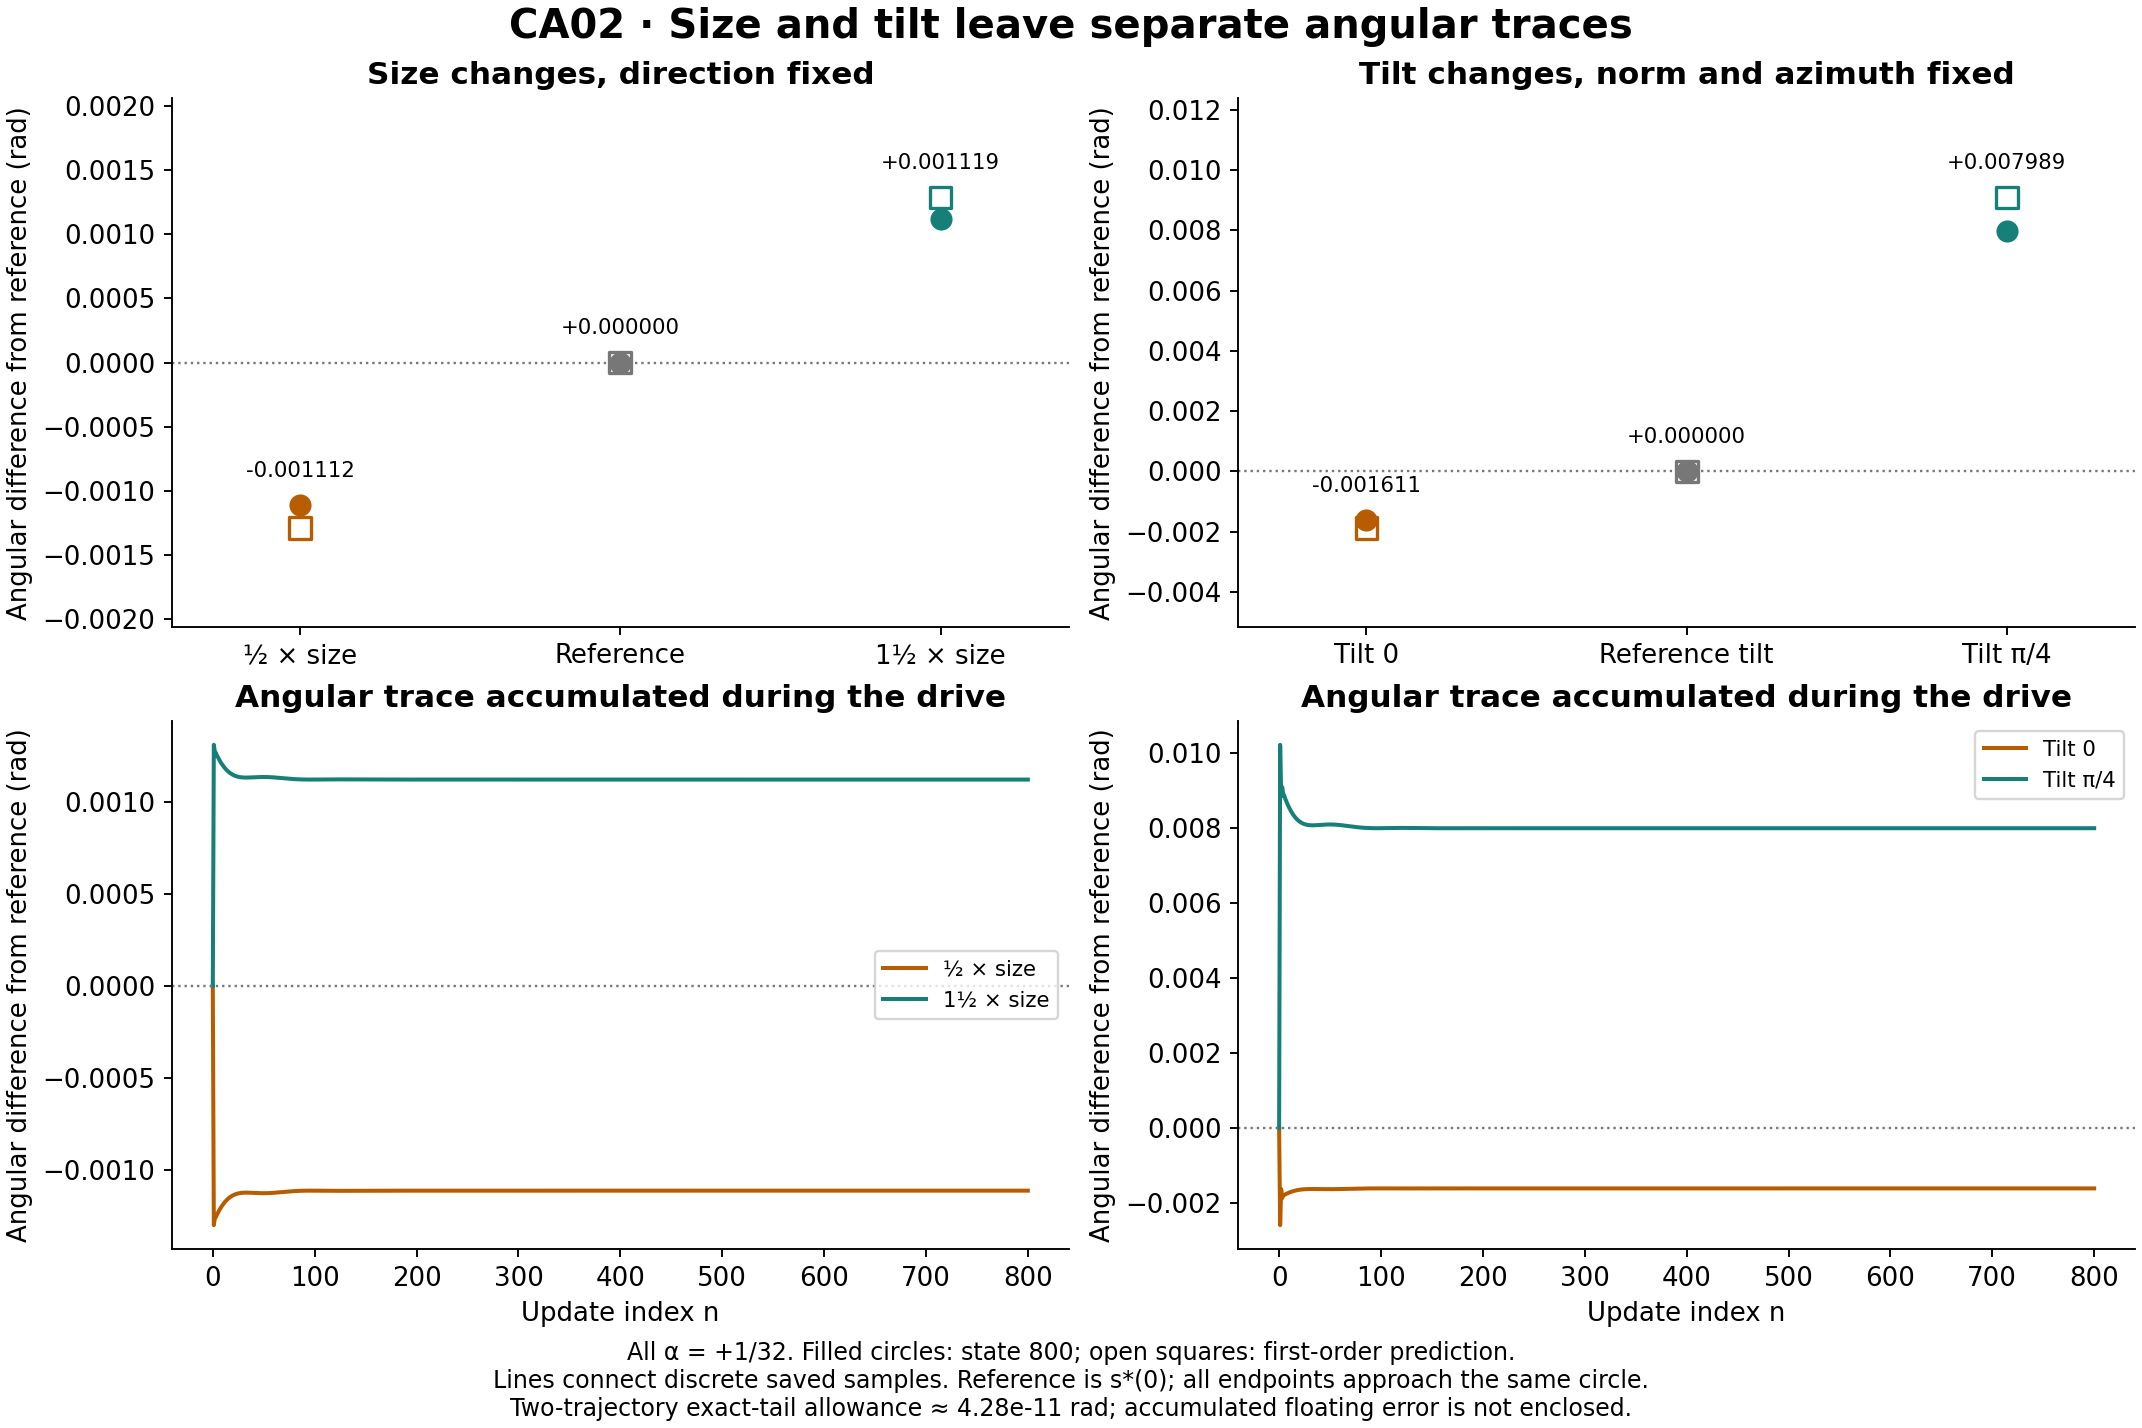
\includegraphics[width=\linewidth,height=0.80\textheight,keepaspectratio]{figures/03_retention.png}
\caption{Separate starting-size and equal-norm starting-tilt comparisons under fading drive. Unchanged CA02 figure \texttt{figures/02\_size\_and\_tilt.png}. The displayed nonzero-coupling values are finite numerical observations with declared diagnostic inputs. The analytic first derivatives establish distinct limiting phases for sufficiently small nonzero coupling; they do not certify every displayed finite-coupling value.}\label{fig:retention}
\end{figure}
\end{landscape}

\section{When the drive returns}\label{sec:return}
\subsection{Returning the input without resetting the state}
The endpoint theorem uses an absolutely summable input. Indefinitely repeating a nonzero input block removes that hypothesis. The appropriate object becomes the full block map, rather than the fading-drive endpoint. CA03 starts from eight exact saved binary64 checkpoints at index 800 of CA02. For local continuation index $j=0,\ldots,2399$, absolute state index is $800+j$, while the forcing index is
\begin{equation}\label{eq:schedules}
f_j=800+j\quad\hbox{(CONTINUE)},\qquad
f_j=j\bmod800\quad\hbox{(RETURN)}.
\end{equation}
In both schedules the current evolving state is carried forward through the complete update. RETURN resets only the forcing index after each block. There is no projection onto the limiting circle and no restoration of an initial state.

The saved three-block comparison makes a restricted but useful observation. Relative to the same reference history, all four selected size/tilt traces remain nonzero and shrink under RETURN (Table~\ref{tab:return}). Their fractions after one, two and three blocks are approximately $0.8591$, $0.7373$ and $0.6320$, respectively, with small differences among cases. CONTINUE changes the corresponding differences by at most $6.68\times10^{-15}$ in the saved calculation. The latter is numerical stability at the displayed resolution, not a proof of exact equality. Figure~\ref{fig:return} presents the saved trace comparison.

\begin{table}[htbp]
\centering\small
\caption{Finite contraction of inherited angular traces over three RETURN blocks at $\alpha=1/32$. Differences are relative to the reference history. Values are saved numerical observations from CA03.}\label{tab:return}
\begin{tabular}{lrr}
\toprule
Comparison & Final angular difference (rad) & Final / initial difference \\
\midrule
Half-size & $-0.000702991202$ & 0.632084274 \\
Three-halves-size & $+0.000707461627$ & 0.632007141 \\
Equal-norm tilt $0$ & $-0.001018539820$ & 0.632101495 \\
Equal-norm tilt $\pi/4$ & $+0.005046949205$ & 0.631768220 \\
\bottomrule
\end{tabular}
\end{table}

The motion during a block is not confined to $\Cset$. The selected saved trajectories reach a maximum distance of about $0.00819863$ from it within a block and return close to it at a boundary. Likewise, different cardinal starting phases respond differently: the saved reference final angle is about $0.112816$, while other cardinal controls end near $0.870489$, $2.830628$ and $5.509202$. These finite observations are consistent with the phase dependence in $G$. They do not establish a common future for every phase or a global attraction region.


\subsection{Six separately defined disturbances}
The inherited disturbance test begins from the original reference CA02 checkpoint, not from a later state in the three-block history. It applies one positive and one negative disturbance of amplitude $\eta=10^{-4}$ in each of three coordinates: fractional size, tilt angle, and phase angle. Each perturbed state then receives one complete returning block. These six operations are separate interventions, with different units; they are not a pooled noise experiment.

The final phase offsets have magnitudes about $1.9141\times10^{-7}$ for fractional-size changes, $1.0756\times10^{-6}$ for tilt changes, and $8.59218\times10^{-5}$ for phase changes. The corresponding saved central tangent estimates are approximately $0.00191410$, $0.0107562$ and $0.859218$ per unit of their respective disturbance parameters. They show that later size and tilt disturbances can also transfer into phase during a return. One amplitude and one checkpoint do not establish robustness to arbitrary noise, an invariant sensitivity law, or a global ordering of disturbance effects. Figure~\ref{fig:disturbance} preserves that scope.


\subsection{A small-coupling theorem for the complete block}
Write the returning $N$-step map in both intrinsic coordinates as $T_\alpha(\theta,\varphi)=(M_\alpha,A_\alpha)$, where $N=800$. Starting on $\Cset$, the accepted first-order block response is
\begin{equation}\label{eq:blockfirst}
A_\alpha(\theta_*,\varphi)=\varphi+\alpha K_NG(\varphi)+O(\alpha^2),\qquad
K_N=\tfrac1{10}\sum_{f=0}^{N-1}H(f/10).
\end{equation}
The differentiated remainder is controlled locally. Geometric sums give a closed expression by replacing every $1/(1-w)$ in~\eqref{eq:S} with $(1-w^N)/(1-w)$. The accepted analytic bound gives $K_{800}>0.15$; its saved estimate is $6.58649686916413$. The sign, rather than the displayed decimal precision, is what the theorem needs.

The leading angular response $G$ has exactly two simple zeros on the circle, one in quadrant I and one in quadrant III. At such a zero,
\begin{equation}\label{eq:rootderivative}
G'(\varphi)=z_*\cos^2\varphi-\frac{\rho_*}{\cos\varphi}.
\end{equation}
It is negative at the first root and positive at the second. Appendix~\ref{app:block} records the algebraic root count and the full two-coordinate reduction.

\begin{theorem}[Local block branches near zero coupling]\label{thm:smallalpha}
For sufficiently small positive $\alpha$, the full 800-update RETURN map has a locally attracting fixed-point branch associated with the quadrant-I zero of $G$, and a saddle branch associated with its quadrant-III zero. For sufficiently small negative $\alpha$, their angular stability is reversed. This theorem supplies neither a quantitative coupling threshold nor a global count of all finite-coupling fixed points.
\end{theorem}
\begin{proof}
At zero coupling, $T_0=(g^N(\theta),\varphi)$, with meridional multiplier $\mu=(\sqrt3-2)^N$. Since $\mu\ne1$, the implicit function theorem solves $M_\alpha(\theta,\varphi)-\theta=0$ locally as $\theta=h(\alpha,\varphi)$. The reduced fixed-point equation is $[A_\alpha(h(\alpha,\varphi),\varphi)-\varphi]/\alpha=0$, smoothly extended to $\alpha=0$ with value $K_NG(\varphi)$. Its two simple zeros give two local full-map fixed-point branches. Their multipliers are $\mu+O(\alpha)$ and $1+\alpha K_NG'(\varphi)+O(\alpha^2)$. The signs above yield the stated stability for sufficiently small coupling of either sign.
\end{proof}

The graph $\theta=h(\alpha,\varphi)$ solves one fixed-point equation; it has not been shown to be an invariant graph for arbitrary iteration. The meridional multiplier $\mu$ is extremely small but strictly positive for even $N=800$; its saved scale is about $2.77\times10^{-458}$. Replacing it by exact zero changes the mathematics. The leading phase estimates, about $0.245118$ and $3.252360$, are likewise not certified finite-coupling roots. In particular, this local theorem does not by itself prove stability at $\alpha=1/32$, connect a finite-coupling root to one of its branches, or establish global convergence. The next section addresses the first of those gaps directly.

\begin{landscape}
\begin{figure}[p]
\centering
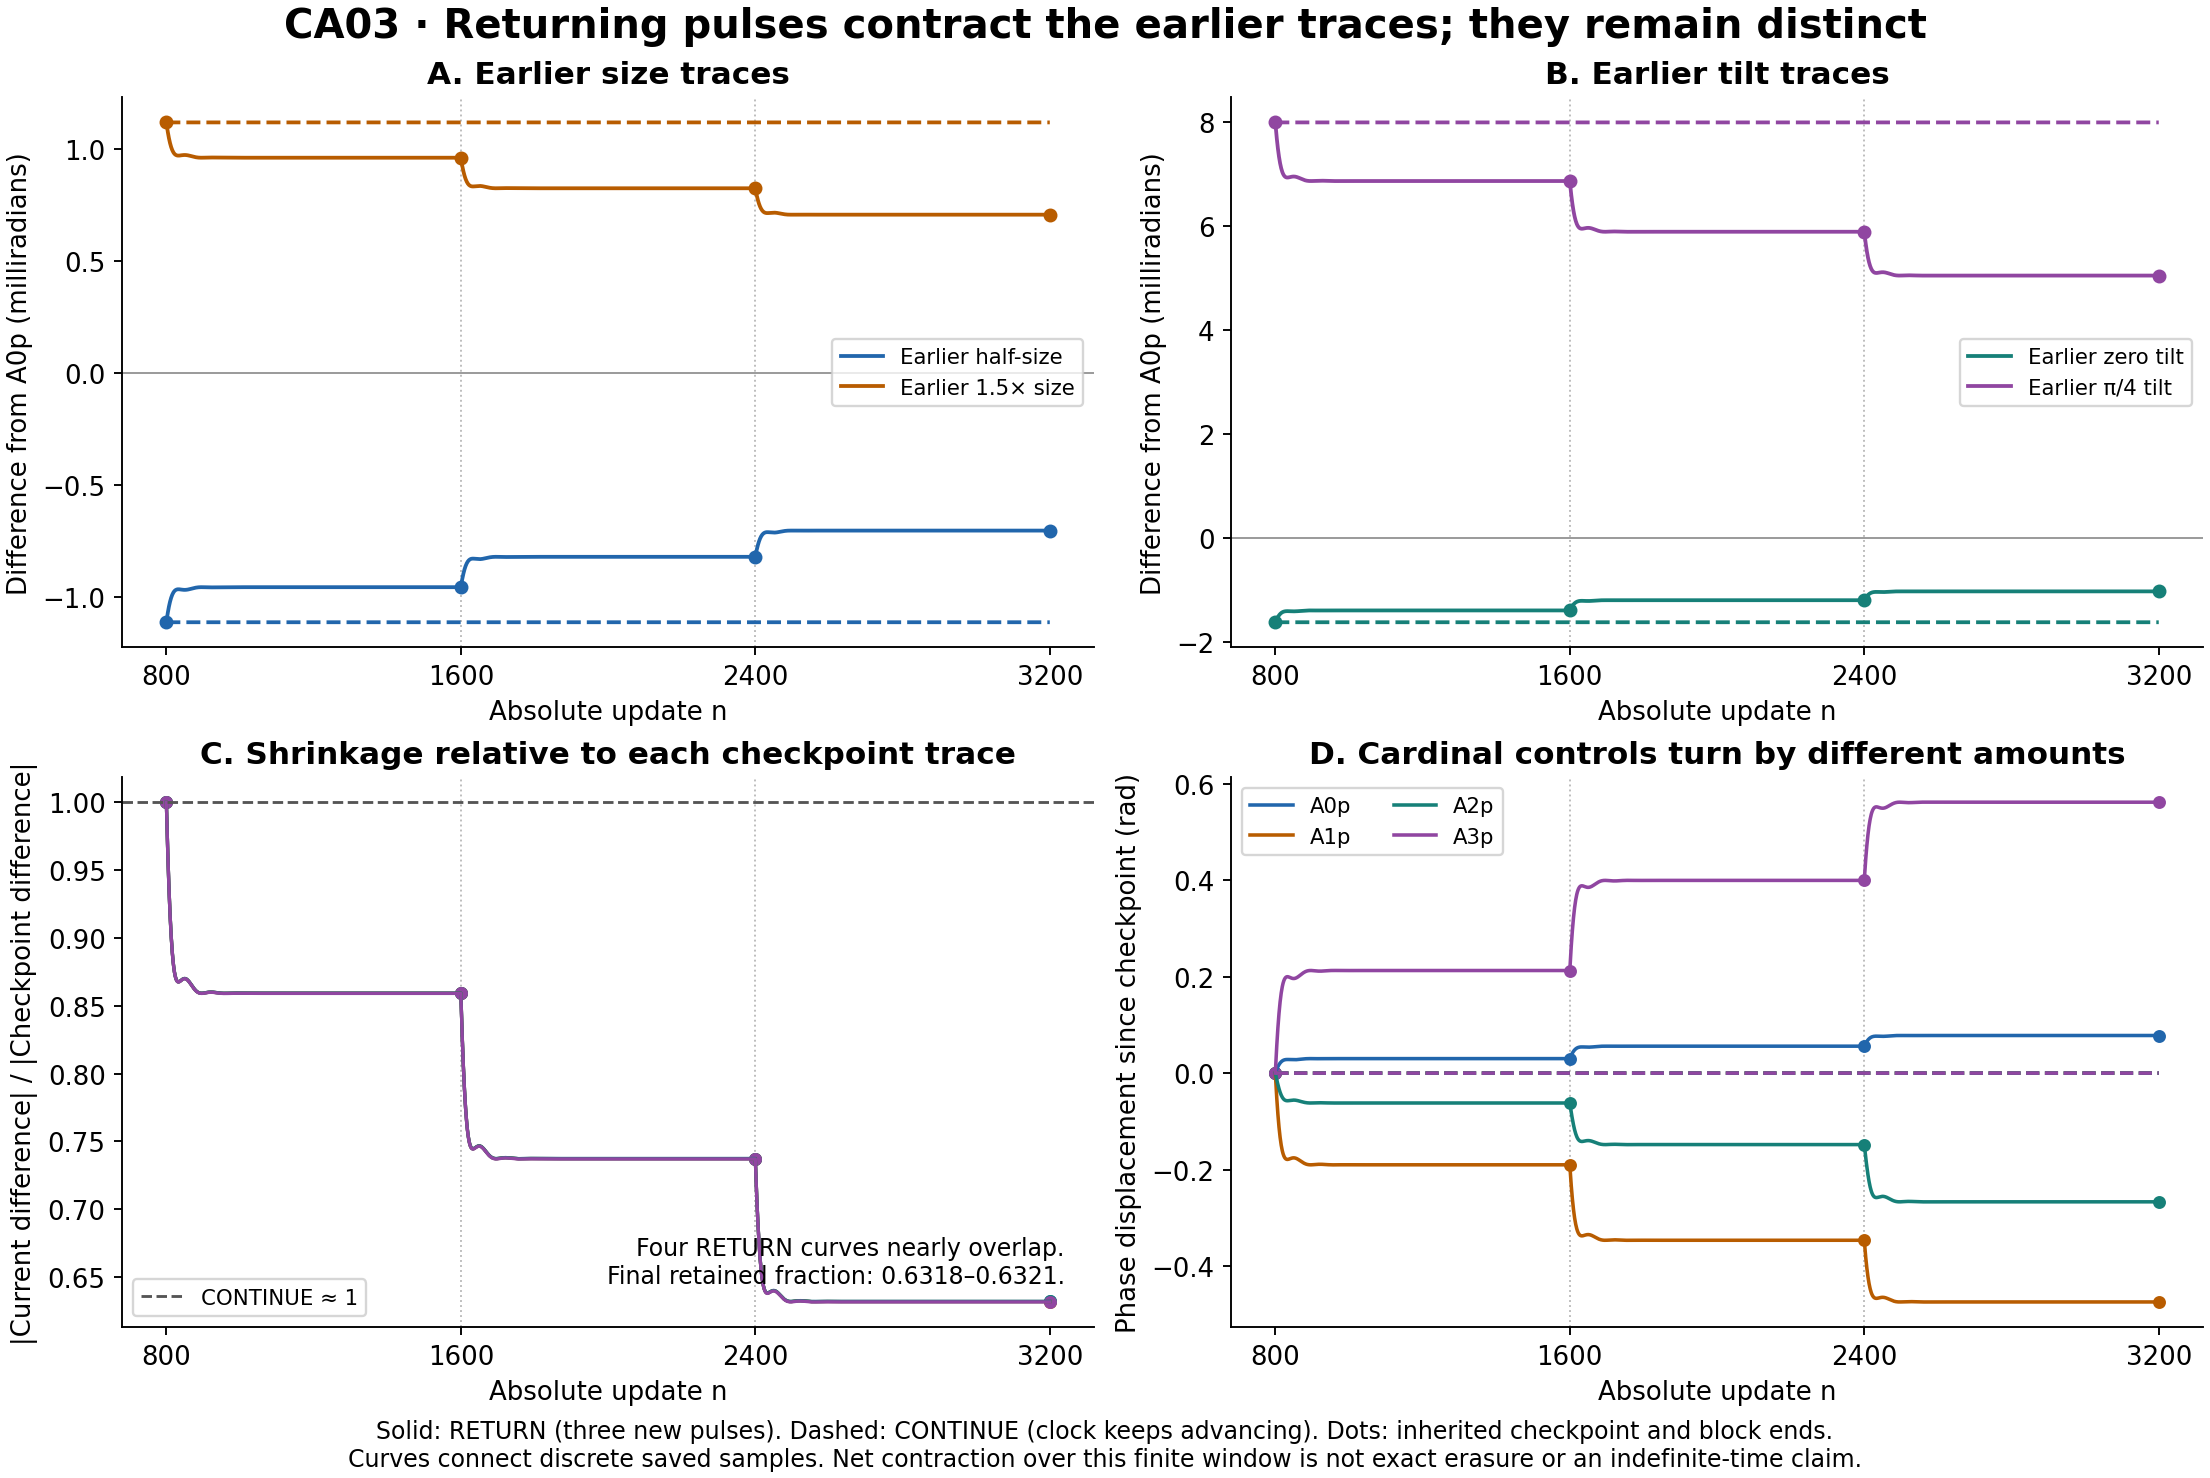
\includegraphics[width=\linewidth,height=0.80\textheight,keepaspectratio]{figures/04_return.png}
\caption{Survival and finite contraction of saved angular traces. Unchanged CA03 figure \texttt{figures/01\_trace\_survival.png}. CONTINUE advances the forcing index; RETURN repeats the 800-value schedule while carrying the current state. Three blocks reduce the selected differences but do not erase them exactly. Indefinite convergence requires the separate theorem and entry certificate in Section~\ref{sec:certificate}.}\label{fig:return}
\end{figure}
\end{landscape}

\begin{landscape}
\begin{figure}[p]
\centering
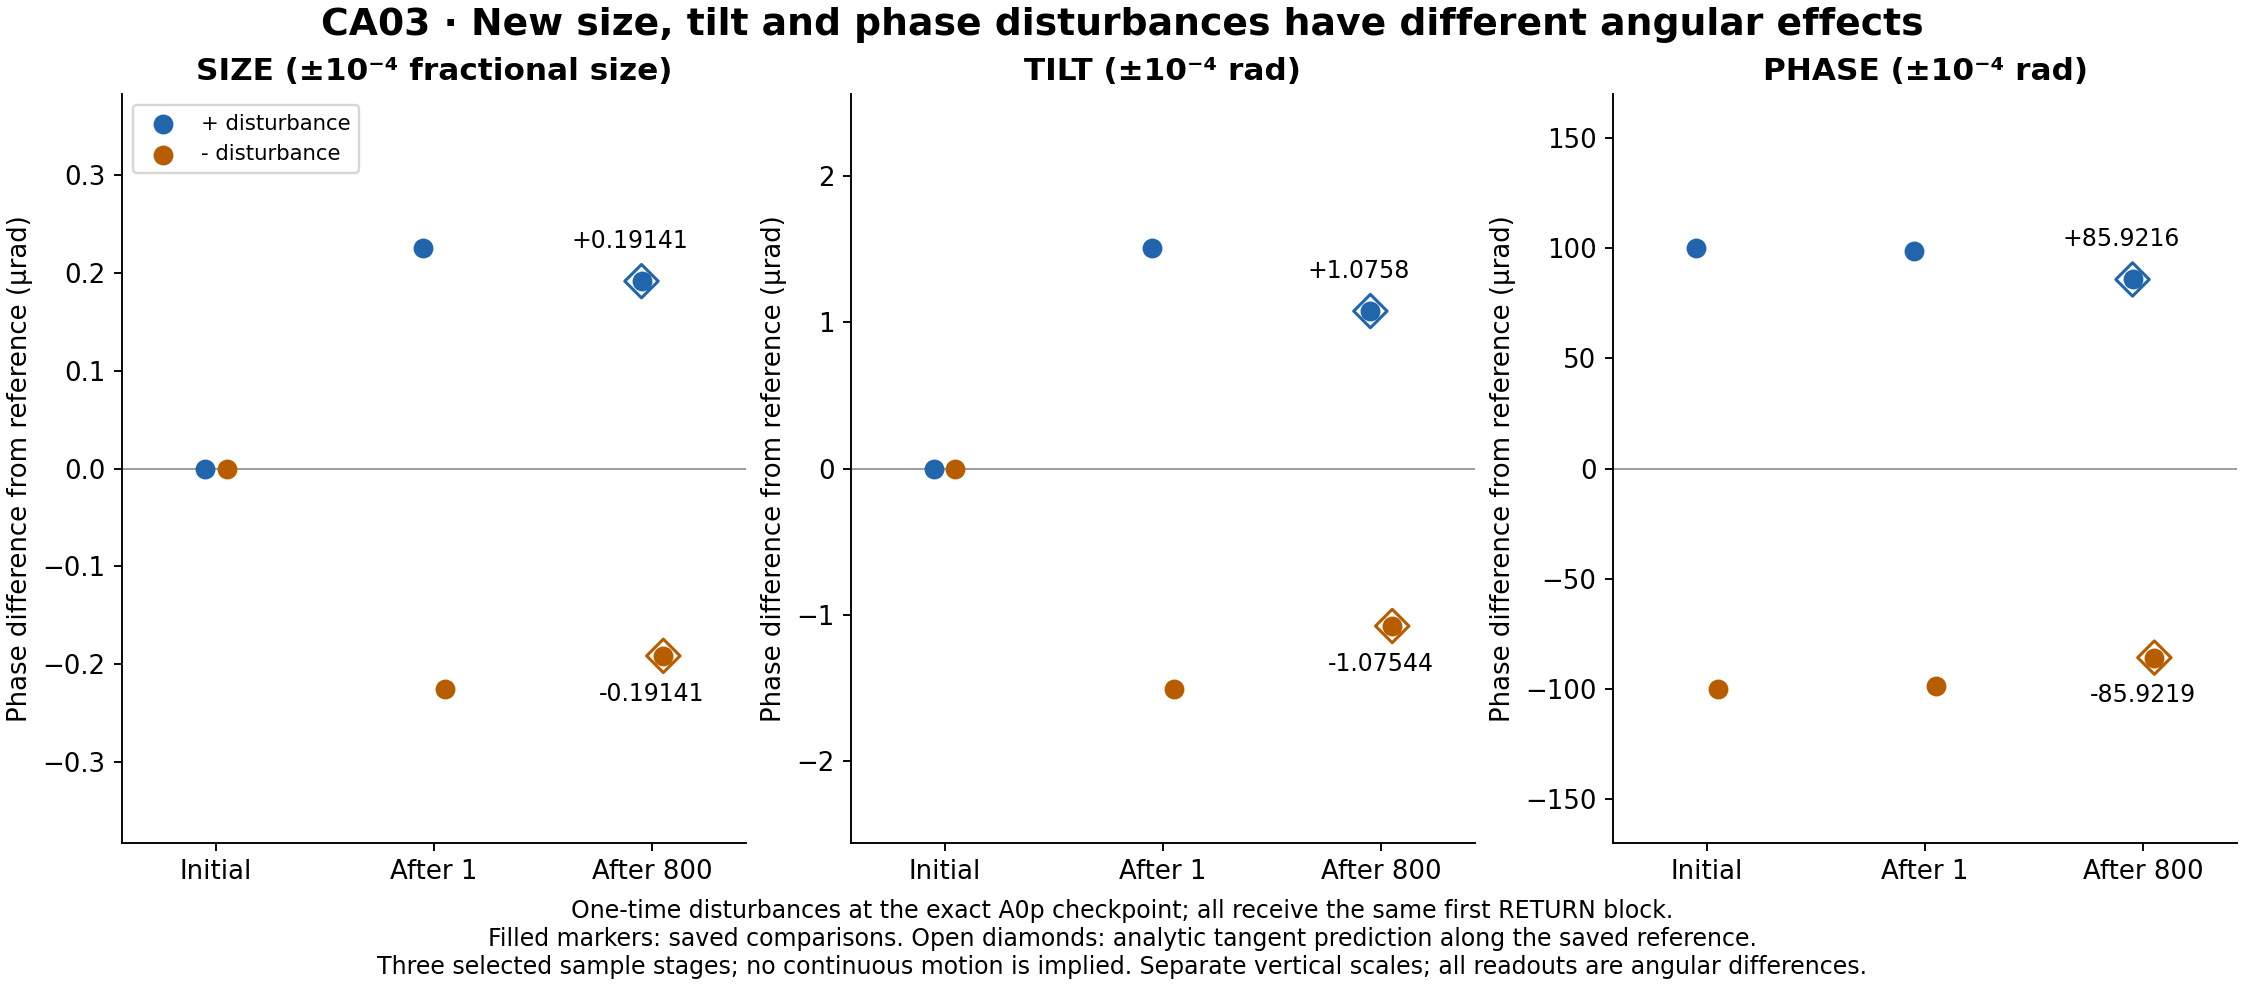
\includegraphics[width=\linewidth,height=0.80\textheight,keepaspectratio]{figures/05_disturbance.png}
\caption{Six local disturbance tests at the saved reference checkpoint. Unchanged CA03 figure \texttt{figures/03\_later\_disturbances.png}. Size, tilt and phase have different parameter units; each signed disturbance is followed by one returning block. These finite responses do not establish a general noise model or an infinite-time conclusion.}\label{fig:disturbance}
\end{figure}
\end{landscape}

\section{Certified convergence at exactly one coupling strength}\label{sec:certificate}
\subsection{The exact target and its two-coordinate chart}
The certificate concerns the exact-real composition of all 800 updates with $\alpha=1/32$, step $1/10$, and forcing times $f/10$ for integers $f=0,\ldots,799$. The same schedule is then repeated indefinitely without resetting the state. No late forcing term is dropped. The state may move off the limiting circle during a block; both surface coordinates are retained.

On $K$, $|H|\le4.5$ and $\|A\|\le9/4$ imply
\begin{equation}\label{eq:clipcertificate}
\|q\|\le\frac{81}{256}<\frac45-\frac1{100000},\qquad
\rho(u)\ge\frac{1199}{2560}>0.
\end{equation}
Thus the full printed clipping operation is present but provably inactive for these on-surface updates. Appendix~\ref{app:arithmetic} explains the $4.5$ bound. This is a branch proof for the target map, not an undocumented replacement of clipping.

The chart used for the certificate is
\begin{equation}\label{eq:chart}
\chi(c,v)=\left((1+c/2)\frac{1-v^2}{1+v^2},\ (1+c/2)\frac{2v}{1+v^2},\ \frac12\sqrt{1-c^2}\right),
\end{equation}
where $c=\cos\theta$ and $v=\tan(\varphi/2)$. The positive square root selects the upper surface. The chart is local in azimuth and excludes its half-angle pole. If $u$ is the Cartesian pre-remap state, the exact coordinate update is $c^+=u_z/\|u\|$ and $v^+=u_y/(\rho(u)+u_x)$ on the validated domain.

For transparent evaluation without repeated angle calls, the accepted equivalent expression introduces $r=1+c/2$, $z=\tfrac12\sqrt{1-c^2}$, $C_v=(1-v^2)/(1+v^2)$ and $S_v=2v/(1+v^2)$. Define
\begin{equation}\label{eq:chartstep}
\begin{aligned}
R_t&=z^2S_v-rzC_v^2,& W_t&=z^2C_v-r^2S_v+rzS_vC_v,\\
Z_t&=r^2C_v^2-rzS_v,& k_f&=H(f/10)/320,\\
a_r&=r+k_fR_t,& b_t&=k_fW_t,\quad d_z=z+k_fZ_t,\\
h_r&=\sqrt{a_r^2+b_t^2},& L_u&=\sqrt{h_r^2+d_z^2},\quad w_t=\frac{b_t}{h_r+a_r},\\
c^+&=d_z/L_u,& v^+&=\frac{v+w_t}{1-vw_t}.
\end{aligned}
\end{equation}
The subscripts distinguish these temporary quantities from the response function $W$ and from the roll $C$. Their equivalence follows by resolving the Cartesian increment into radial and tangential components and applying the half-angle addition identity. The certificate encloses all square-root arguments and denominators, verifies the positive branches, and keeps $-1<c<1$ throughout. The explicit graph matters because differentiating a different map would not certify the printed recurrence.

\subsection{Two regions and a contraction argument}
The accepted rational centre is
\begin{equation}\label{eq:center}
\widehat x=(\widehat c,\widehat v)=
\left(\frac{3296863744182679}{9007199254740992},\ 
\frac{4382175857337591}{36028797018963968}\right).
\end{equation}
It is approximately $(0.3660254037843512,0.1216298133693170)$. Define coordinate boxes $X$ and $B$, both centred at $\widehat x$, with exact rational radius vectors
\begin{equation}\label{eq:radii}
r_X=(10^{-6},10^{-5}),\qquad r_B=(10^{-3},10^{-1}).
\end{equation}
The smaller region localizes the root; the larger region establishes a useful entry neighbourhood. Neither is a ball drawn around a trajectory. They are explicit domains in a two-dimensional chart of the map's actual surface.

For $Y=X$ or $B$, the certificate encloses the centre residual componentwise by $e\ge|T(\widehat x)-\widehat x|$ and the full-domain Jacobian by a nonnegative matrix $M_Y\ge|DT(x)|$ for all $x\in Y$. The essential checks are
\begin{equation}\label{eq:certificateineq}
e+M_Yr_Y<r_Y,\qquad
q_Y=\max_i\frac{(M_Yr_Y)_i}{(r_Y)_i}<1.
\end{equation}
The first is a strict interior-inclusion proof; the second is contraction in the weighted maximum norm $\|h\|_{r_Y}=\max_i|h_i|/(r_Y)_i$. These checks concern the actual block map, not the convergence of a Newton solver used to find a candidate.

\begin{table}[htbp]
\centering\small
\caption{Readable summaries of accepted CA04 certificate bounds. Matrix entries are coarser upward displays; $q$ values summarize the original saved enclosures. The proof inputs are the exact endpoints in \texttt{CERTIFICATE.json}, not the rounded table.}\label{tab:certificate}
\begin{tabular}{lcc}
\toprule
Quantity & $X$ & $B$ \\
\midrule
$M_{11}$ upper display & $3.304\times10^{-16}$ & $2.691\times10^{-15}$ \\
$M_{12}$ upper display & $1.464\times10^{-13}$ & $4.244\times10^{-13}$ \\
$M_{21}$ upper display & $0.001919$ & $0.005490$ \\
$M_{22}$ upper display & $0.850415$ & $0.924524$ \\
Automatic derivative $q$ & $0.850606416789<0.851$ & $0.924578804694<0.925$ \\
Separate hand derivative $q$ & $0.850607383690<1$ & $0.943681887849<1$ \\
Second-coordinate inclusion margin & $1.49394\times10^{-6}$ & $0.00754212$ \\
\bottomrule
\end{tabular}
\end{table}

The saved residual bounds are approximately $e_1=2.90090\times10^{-18}$ and $e_2=1.58224\times10^{-16}$. A small residual alone would not establish the conclusion: it is combined with full-region derivative and domain bounds. The hand-differential route produces wider enclosures than automatic differentiation, especially on $B$, but independently satisfies the same sufficient contraction criterion. Different valid enclosure widths are not inconsistent results.

\begin{theorem}[Accepted exact-real return certificate]\label{thm:certificate}
For the complete RETURN map specified above at exactly $\alpha=1/32$, there is a unique fixed point in $X$ and a unique fixed point in $B$, and these points coincide. Every initial coordinate point in either region converges under indefinite block iteration to that fixed point. This is local attraction on the two-dimensional intrinsic surface, not a global or ambient three-dimensional basin theorem.
\end{theorem}
\begin{proof}
The accepted outward arithmetic establishes the map's domain and the inequalities~\eqref{eq:certificateineq} throughout both boxes. The mean-value bound gives $T(Y)\subset\operatorname{int}Y$. The derivative bound gives a Lipschitz constant $q_Y<1$ in the stated weighted norm on the convex, complete box. The contraction mapping theorem supplies existence, uniqueness and convergence in each box. Since $X\subset B$, the fixed point in $X$ is also in $B$ and uniqueness there identifies the two.
\end{proof}

The accepted a posteriori bound $(I-M_X)^{-1}e$ further localizes the root. Its phase satisfies
\begin{equation}\label{eq:rootphase}
0.2420705842886754<\varphi_*<0.2420705842886798.
\end{equation}
The saved coordinate errors relative to the rational centre are less than $2.901\times10^{-18}$ in $c$ and $1.058\times10^{-15}$ in $v$. A Cartesian estimate, rounded for display, is
\begin{equation}\label{eq:rootcart}
s_{\rm return,*}\simeq(1.14852044,\ 0.28358394,\ 0.46530243).
\end{equation}
These readouts are inherited consequences of the exact bounds. They were not recomputed for this manuscript. In particular, the result does not prove that this root is the analytic continuation of a specific small-coupling branch, or that its repeating response has minimal period 800.

\subsection{Entry of five exact saved states}
The entry extension starts from the five final RETURN states indexed in the accepted CA04 input index: raw CA03 state array row 2400, corresponding to absolute update index 3200. Each saved binary64 component is interpreted as its exact dyadic real value. These are precisely specified new initial conditions, not rounded endpoint-table reconstructions. Their future forcing starts at $f=0$.

The Cartesian input can differ slightly from the exact remapped surface because its past was computed in floating point. The entry proof therefore applies the actual first Cartesian update, including clipping and axis checks, before using intrinsic coordinates for forcing indices $1$ through $799$. It does not fit or project the saved point onto a circle or torus before that first update. After one complete block, all five enclosures lie in $B$ (Table~\ref{tab:entry} and Figure~\ref{fig:certificate}).

\begin{table}[htbp]
\centering\small
\caption{Accepted one-block entry results for five exact dyadic inputs. The shown $v$ values are readable summaries of interval enclosures, each of width less than $2\times10^{-45}$. Full component ratios and endpoint bounds are retained in the supplementary CA04 input index and certificate.}\label{tab:entry}
\begin{tabular}{lll}
\toprule
Source ID & Initial comparison lineage & Enclosed final $v$, approximately \\
\midrule
\texttt{A0p} & Reference history & 0.065973712572206 \\
\texttt{Bhalf} & Half-size history & 0.065671414263580 \\
\texttt{Bthreehalf} & Three-halves-size history & 0.066277935162302 \\
\texttt{Czero} & Equal-norm tilt $0$ history & 0.065535723538212 \\
\texttt{Cquarter} & Equal-norm tilt $\pi/4$ history & 0.068144045826960 \\
\bottomrule
\end{tabular}
\end{table}

\begin{corollary}[Certified futures of the indexed states]\label{thm:entry}
Under the specified indefinite RETURN schedule at $\alpha=1/32$, the five exact saved inputs converge at block boundaries to the same certified fixed point. At each fixed within-block phase they converge to the corresponding phase of its repeating response.
\end{corollary}
\begin{proof}
The accepted entry enclosures place all five one-block images in $B$. Theorem~\ref{thm:certificate} then gives convergence at block boundaries. Every fixed finite prefix of the block is continuous on the validated orbit neighbourhood, so applying that prefix to the converging boundary states gives convergence at the corresponding within-block phase.
\end{proof}

Convergence is asymptotic. It does not assert equality after finitely many blocks, erase the documented finite differences retroactively, or certify the unknown exact real trajectories preceding the stored binary64 inputs. Nor does it cover the other cardinal controls, negative-coupling controls, all size and tilt states, or arbitrary noisy perturbations. This separation between finite historical evidence and newly specified exact futures is central to the interpretation of the result.

\begin{landscape}
\begin{figure}[p]
\centering
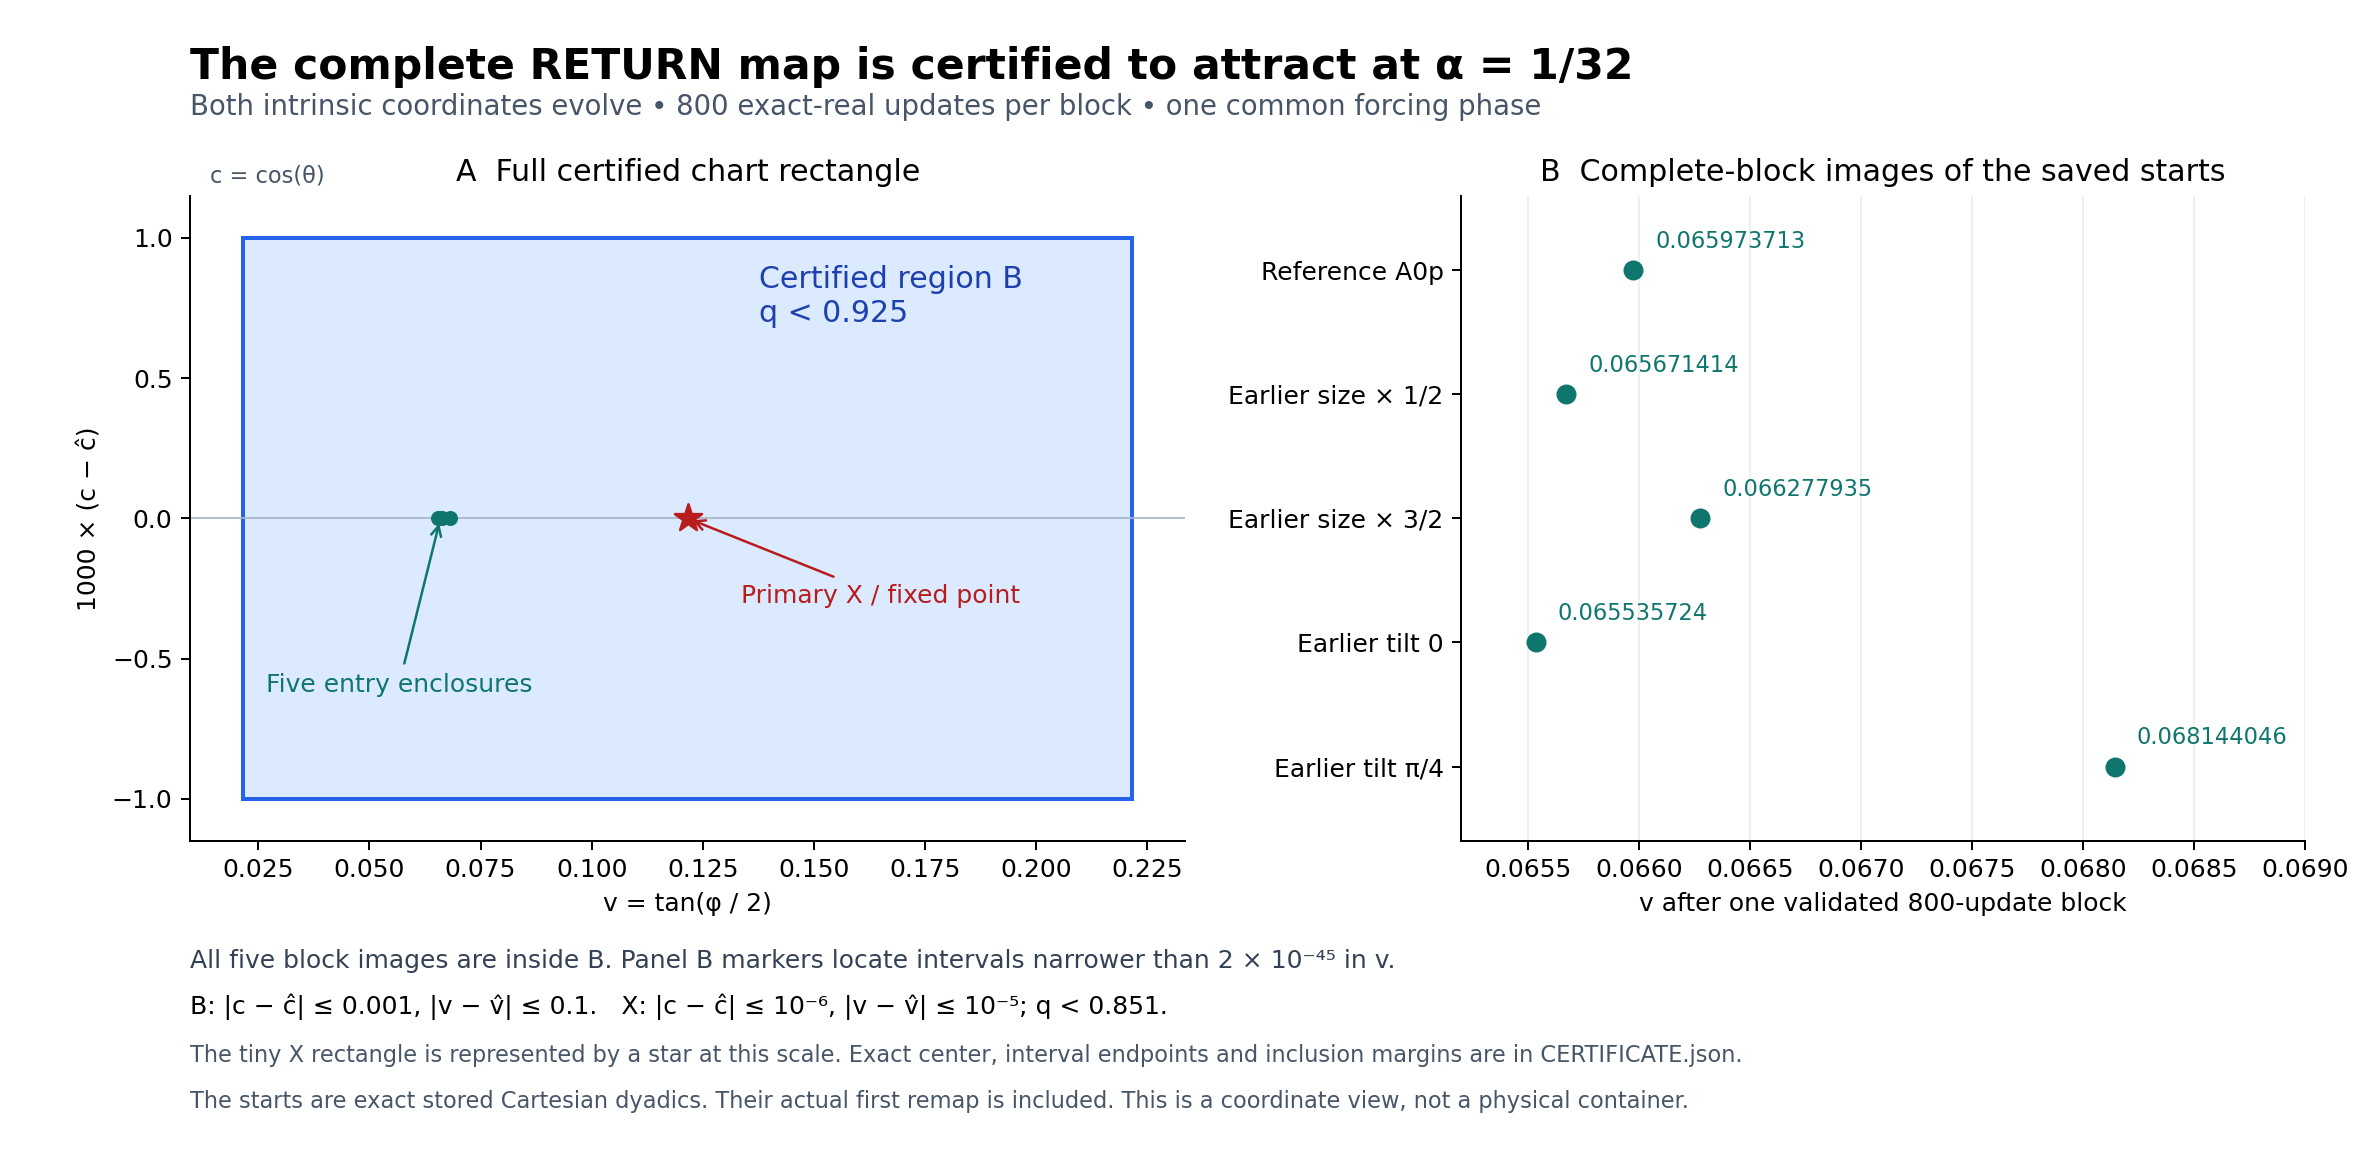
\includegraphics[width=\linewidth,height=0.80\textheight,keepaspectratio]{figures/06_certificate.png}
\caption{Certified regions and entry of the five indexed states. Unchanged CA04 figure \texttt{figures/CA04\_certified\_region\_and\_entry.png}. The image illustrates exact bounds stored in the certificate; drawing a region does not prove inclusion. The accepted inequalities establish contraction in both intrinsic coordinates, and the separate Cartesian-first entry proof places each exact saved input in the larger region after one block.}\label{fig:certificate}
\end{figure}
\end{landscape}

\subsection{Arithmetic and review: what is trusted}
The certificate uses task-specific outward interval arithmetic with exact integer endpoints on a $2^{-160}$ grid. Rational conversion, signed arithmetic, reciprocal, squaring and integer-square-root bounds enclose exact results. All 800 forcing values are enclosed using reduced-argument Taylor series and exact remainder bounds. Signed derivative enclosures are propagated through the complete composition before taking componentwise absolute bounds. The verified domains require no subdivision in the accepted certificate. Appendix~\ref{app:arithmetic} gives the construction and the separate hand-differential check.

The accepted scientific review inspected these constructions and ran the fixed verifier once in a separate copy, accounting for 8000 interval set-step evaluations. A separately implemented reviewer checker constructed another rigorous enclosure of every forcing value using 224-bit rational endpoints and a different Taylor/reduction configuration; each of its 800 enclosures lay inside the submitted one. It also checked exact rational contraction and localization implications, input identities and saved relations \cite{review04}. Those are prior review actions, not computations performed for this paper.

The trust boundary remains explicit. The submitted verifier and its automatic and hand derivative routes share the reviewed integer interval core. The reviewer forcing construction and rational checks are separately implemented, but there is no wholly independent second end-to-end state-and-derivative certificate, and no proof-assistant formalization. The result is a transparent exact-real computer-assisted proof conditional on the reviewed implementation of exact integer arithmetic and the stated mathematical bounds. Calling it a certificate does not remove those implementation assumptions; treating it as a high-precision trajectory would understate what its enclosure inequalities establish.

\section{Interpretation through a passive geometric reference}\label{sec:geometry}
The accepted reference geometry can organize views, distances and orientation conventions without contributing an update. CA01 used the accepted width-one Tri-Octagon host and, separately, the refined zero-member PLUS/MINUS crystal face complexes. Each crystal complex has 18 vertices, 24 triangular faces, 42 edges and two open six-edge boundary cycles. The two crystal hands share the zero-member vertex set but have different face surfaces. These data were taken from the accepted source, not reconstructed from a sketch or a photograph. Nothing in the arguments above requires an invented central ball or a closed physical shell.

The recorded observer placement uses unit scale and offset $O=(0,\sqrt3/6,0)$. Reporting $O+s$ in that reference changes a placement, not the recurrence. A passive orthogonal change of frame rotates both data and reference axes. Native coordinates and Euclidean distances then represent the same state and relations. By contrast, actively rotating only a starting state while leaving $C$ unchanged creates a different driven experiment. Under a genuine coordinate transformation, the roll is represented by $QCQ^{-1}$, not silently kept fixed. This is why apparent changes between views must be separated from changes of the operator.

The measurement framework adds three useful questions: where is the reference origin, which coordinates are native to the dynamics, and which features survive a change of view? It helps expose that a centroid can lie far from every selected field point, and that a visually central marker can be a statistic rather than a moving object. It can also display departures from the remapping surface or the limiting circle. It does not establish an SRG-to-Z relation, generate a force, close the accepted mesh's openings, or make an unproved orbit physically confined.

In this study, the strongest dynamics are visible without a complex overlay: one neutral angular coordinate under zero drive, summable angular changes under fading drive, and a certified contraction of both chart coordinates under a returning schedule in a local region. The framework is most useful when it makes those distinctions clearer. It becomes misleading if a desired shape is used to choose or modify the trajectory. No such fitting or modification is part of the accepted results or this paper.

\section{Conclusions and limits}\label{sec:conclusion}
The historical figures motivate different mathematical questions. Figure 3's central marker is a field statistic whose exact symmetry can fix it at the origin; its movement in finite arithmetic need not describe attraction. Figure 4 carries a genuine state through a complete driven recurrence. Its remapping attracts to a circle as a set, while leaving angular position neutral in the unforced limit.

An advancing fading drive preserves that endpoint family but changes which endpoint a given initial state reaches. Size and tilt can affect the angular coordinate before their direct representation is removed. The accepted analytic comparisons prove both transfer mechanisms for sufficiently small nonzero coupling; the saved finite diagnostics show distinct traces at their declared settings. Retention is selective rather than complete: a single endpoint angle cannot generally encode an entire three-dimensional initial state.

Returning the drive changes the asymptotic problem. The inherited three-block observations establish finite contraction of selected differences. The small-coupling theorem explains local attracting and saddle branches but leaves its coupling range unquantified. The exact-real certificate then resolves a specific finite-coupling question: at $\alpha=1/32$, the complete 800-update RETURN map is a contraction on the specified regions and has one fixed point there. The entry proof connects five exact saved inputs to that result. Their indefinitely repeated futures converge to the same repeating response, while their finite past differences remain real features of the saved observations.

The conclusions are local where the proofs are local. They do not establish global attraction, minimal period, attraction for all phases or coupling values, or certification of the unknown exact histories behind floating-point checkpoints. The historical producer and run settings remain incomplete. No heat, entropy, temperature, magnetic or light-storage claim is established here; those questions require separate definitions and evidence and are not adjudicated by this dynamical analysis. The geometric framework remains an analytical instrument throughout.

\section*{Data, code and preparation statement}
\addcontentsline{toc}{section}{Data, code and preparation statement}
The publication package includes this PDF, editable TeX, synchronized Markdown, the six reused figures, bibliography, claim/source ledger, symbol crosswalk, source lineage, publication record and source-preservation summary. Four accepted review archives and their scientific-review reports and independent-review archives are retained unchanged in \texttt{supplement/}. Selected analyses and saved tables are exposed in \texttt{sources/} for convenient inspection. The accepted CA04 archive contains the standalone scientific verifier; it is retained as evidence and was not executed during manuscript preparation. A separate editorial build helper synchronizes text and compiles the document; preparation also checks source and figure hashes. No new scientific result is claimed from that preparation.

\section*{Acknowledgments}
\addcontentsline{toc}{section}{Acknowledgments}
GPT contributed scientific direction and internal scientific review in the documented CA01--CA04 workflow. Codex contributed implementation, analysis and manuscript preparation within the authorized work orders. The author is responsible for review and any subsequent decision to submit or publish. No external affiliation, funding award or external reviewer is asserted.

\appendix
\section{Endpoint regularity and the two retention comparisons}\label{app:regularity}
\subsection{Why differentiation through the limiting endpoint is valid}
For a fixed compact neighbourhood of admissible off-axis initial states, restrict $\alpha$ sufficiently close to zero. The first finitely many updates stay in a smooth domain and clipping is inactive there. After a finite entrance time, the meridional derivative is bounded by a constant $r<1$, while the unforced azimuthal derivative equals one. The drive perturbs these derivatives by quantities bounded by a constant times $|\alpha H_n|$. Their neutral-direction products are bounded by
\begin{equation}\label{eq:product}
\prod_n(1+K_0|\alpha H_n|)\le
\exp\left(K_0|\alpha|\sum_n|H_n|\right)<\infty.
\end{equation}
Here $K_0$ is a neighbourhood-dependent bound, distinct from the block sum $K_N$. Variation of constants in the stable direction is a convolution with a geometric kernel. It controls first sensitivities; the stable component decays with summable forcing. For second and third derivatives, differentiation of the unforced meridional map introduces products containing stable sensitivities, while every angular-increment term retains a factor of the summable drive. Induction therefore bounds the differentiated state sequences and makes the angular-increment derivative series converge uniformly through the required orders. Finite initial terms are smooth and cause no infinite-tail difficulty.

This yields a locally $C^3$ endpoint phase and justifies~\eqref{eq:firstresponse}, its Taylor expansion, and the expected second-order accuracy of central differences. It does not provide a numerical bound on the third derivative at a specified finite coupling. The distinction matters: an observed central-difference ratio close to four supports consistency with the expansion but cannot replace its uniform-convergence argument.

\subsection{Scale transfer in the complete clipped update}
Quadratic homogeneity gives $A(\lambda s)=\lambda^2A(s)$. For $\lambda>0$, homogeneity of $P$ rewrites the full first step as
\begin{equation}\label{eq:fullscale}
P\left(s+\tfrac1{10}\alpha H\lambda A(s)
\min\left(1,\frac{4/5}{|\alpha H|\lambda^2\|A(s)\|+1/100000}\right)\right).
\end{equation}
The factor $\lambda$ survives inside the argument. Thus scale erasure by the remapping is compatible with scale-dependent angular transfer before the remapping. Differentiating at zero coupling removes clipping locally, and only the initial $W$ value differs along a positive ray; all later zero-drive iterates agree. Since $H(0)=4.5$, this gives exactly~\eqref{eq:size}. The torque-free diagonal is an exact exception because the whole initial increment vanishes there, not merely its first-order angular component.

\subsection{Strict tilt signs and a controlled scalar tail}
For the tilt family of~\eqref{eq:tilt}, the accepted inequalities use $|H_n|\le4.5$, $|w'|\le5/8$, and the geometric meridional error. The correction from indices $n\ge M$ is bounded by
\begin{equation}\label{eq:tilttail}
\frac1{10}\,4.5\,\frac{5\pi}{16}\,
\frac{3^{-(M-1)}}{1-1/3}.
\end{equation}
The saved $M=40$ calculation includes index zero and correction indices 1 through 39; it is not a sum of 40 nonzero-index correction terms. The displayed derivative estimates in Table~\ref{tab:retention} are inherited from that bounded scalar evaluation.

For $\beta=0$, combining the initial term with the first correction gives a difference bounded above by $0.45(1/4-2b)<-0.0522$. The accepted refinement $|\theta_2-\theta_*|<0.108$, using the local derivative bound $0.27$, limits the remaining contribution by $0.0455625$. The total is strictly negative. For $\beta=\pi/4$, $W_0>0.89$ and $b<0.184$ give an initial difference greater than $0.3177$, while the remaining absolute contribution is bounded by $0.45(5/8)(\pi/6)/(1-1/3)<0.221$. The total is strictly positive. These estimates prove that the two equal-norm tilts lie on opposite sides of the reference first derivative without relying on rounded endpoint plots.

\section{Leading block roots and the full-map reduction}\label{app:block}
With $v=\tan(\varphi/2)$, the equation $G(\varphi)=0$ reduces, away from $\varphi=\pi$, to
\begin{equation}\label{eq:quartic}
bv^4+2(\rho_*+z_*)v^3+2(\rho_*-z_*)v-b=0.
\end{equation}
The coefficient signs and Descartes' rule give one positive and one negative root: for negative arguments apply the same rule to the polynomial in $-v$. Sign changes of $G$ at the cardinal angles place the positive root in quadrant I and the negative-half-angle root in quadrant III. The omitted angle $\pi$ is not a root because $G(\pi)=-b$. Substituting the root equation into $G'=-b\sin\varphi+z_*\cos(2\varphi)-\rho_*\cos\varphi$ gives~\eqref{eq:rootderivative}, which is strictly negative in quadrant I and positive in quadrant III.

At zero drive, the full block retains the contracting meridian. The fixed-point reduction must therefore begin with $M_\alpha(\theta,\varphi)-\theta=0$, whose derivative with respect to $\theta$ is $\mu-1\ne0$. Solving this equation first makes the angular reduction legitimate for fixed points of the two-dimensional block. Simply iterating an angular formula while setting the meridian permanently to $\theta_*$ would define a different map at nonzero coupling. The accepted proof uses the smooth reduced equation only to locate local branches and recover the two full-map multipliers. It makes no invariant-circle claim for the driven map.

The first-order roots, the finite three-block observations, and the certified root are three different objects. Their numerical proximity can motivate a continuation question, but neither a plot nor the local implicit-function argument proves the connection at $1/32$. No branch-following computation or global root search was added for this paper.

\section{Certificate construction and exact-input lineage}\label{app:arithmetic}
\subsection{A uniform drive bound and smooth on-surface updates}
For $t\ge0$, $|\sin t|\le t$ and $|\cos t|\le1$ give a bound for the first two drive terms by $2e^{-t/2}+te^{-3t/10}$. The accepted analysis shows this expression is at most two: its derivative is nonpositive on $0\le t\le10/3$ using $(1-0.3t)e^{0.2t}\le1$, and both derivative terms are nonpositive thereafter. The remaining positive terms sum to at most $2.5$. Hence $|H(t)|\le4.5$. Combining this with the on-surface norm bound proves~\eqref{eq:clipcertificate}; it is sharper than simply adding all four coefficient magnitudes.

The certificate propagates full rectangles through every update of~\eqref{eq:chartstep}. It verifies the arguments of square roots and positivity of $a_r$, $h_r$, $L_u$, $h_r+a_r$, $1-vw_t$, and the equivalent original-chart denominator $h_r+u_x$. These bounds enforce both the local half-angle branch and the algebraic equivalence to the Cartesian remap. Bounding only endpoint values would not suffice: every intermediate map must be defined over the propagated set.

\subsection{Outward arithmetic, forcing and derivatives}
Each interval endpoint is an integer divided by $2^{160}$. Rational input conversion uses floor and ceiling in the appropriate directions. Products consider signed endpoint combinations, reciprocal excludes zero, and square-root endpoints use integer-square-root inequalities. This construction encloses exact real arithmetic without relying on ordinary floating-point round-to-nearest as a proof primitive.

Forcing arguments are exact rationals $f/10$. The submitted forcing engine reduces arguments by 128, uses degree-64 Taylor polynomials with bounds $3/65!$ for the exponential remainder and $1/65!$ for the sine and cosine remainders on the reduced domain, and restores full arguments by seven doubling or squaring identities. Every operation is outward enclosed. The small late forcing values are included rather than set to zero. The separate reviewer engine used degree 96, division by 256 and eight restoration steps with 224-bit rational endpoints. Its containment checks are inherited review evidence, not a fresh execution in this editorial task.

Automatic differentiation propagates a signed $2\times2$ interval Jacobian through all 800 updates over the full domain enclosure. Taking absolute values only after the signed composition retains cancellations needed for useful bounds. A separately derived hand differential supplies a second derivative route, but both use the same interval primitives. The accepted certificate saves their results and the domain checks. The finite test suite and independent rational checks supplement the written general enclosure argument; their Boolean-check count is not a count of mathematical theorems.

The scalar phase enclosure uses $2\arctan v$ and the accepted odd-power series through $j=127$, with remainder bounded by $2/(257\,2^{257})$ on $|v|\le1/2$. The root localization uses the saved nonnegative matrix $M_X$, residual $e$, and the exact rational implication $(I-M_X)^{-1}e$. No displayed rounded phase or matrix in the paper is substituted for these exact proof inputs.

\subsection{Saved states and review reproducibility}
The five input states are identified by file/member names, array index, exact integer ratios and hashes in the accepted \texttt{CA04\_INPUT\_INDEX.json}. The full certificate and its scalar consequences retain the interval endpoints and the links to those inputs. This edition exposes copies of those records in \texttt{sources/CA04/}; the accepted archive remains the authoritative unmodified container. The source lineage records the earlier CA02 checkpoint and CA03 continuation identities without recomputing their prefixes.

For review, the package separates editorial reproduction from scientific verification. Compiling the TeX, comparing copied data hashes, checking the claim ledger and viewing the PDF require no scientific rerun. The accepted standalone verifier remains inside the CA04 archive for a separately authorized review. It was not imported or executed by the manuscript tools. The exact input interpretation, complete forcing schedule, region radii, centre and trust boundary stated here are sufficient to identify precisely which inherited theorem is being reported.

\FloatBarrier
\clearpage
\begin{thebibliography}{99}
\bibitem{historical} Hilmir F. Halldórsson (pzychozen), ChatGPT and Grok. \emph{SGR: simulation steps}. Historical note, 1 August 2025. Title-page credits retained as printed; Figures 3 and 4 and accompanying text, physical pp. 5--8. Supplied file: \texttt{SGR\_simulations.pdf} in the CA01 accepted archive.
\bibitem{ca01} SRG research record. \emph{CA01 source and measurement analysis}, v0.1. Accepted local analysis: \texttt{CA01\_ANALYSIS.md}; archive \texttt{CA01\_GPT\_REVIEW.zip}. Accepted research evidence reproduced in the publication supplement.
\bibitem{ca02} SRG research record. \emph{CA02 endpoint retention analysis}, v0.1. Accepted local analysis: \texttt{CA02\_ENDPOINT\_RETENTION\_ANALYSIS.md}; archive \texttt{CA02\_GPT\_REVIEW.zip}. Accepted research evidence reproduced in the publication supplement.
\bibitem{ca03} SRG research record. \emph{CA03 returning drive analysis}, v0.1. Accepted local analysis: \texttt{CA03\_RETURNING\_DRIVE\_ANALYSIS.md}; archive \texttt{CA03\_GPT\_REVIEW.zip}. Accepted research evidence reproduced in the publication supplement.
\bibitem{ca04} SRG research record. \emph{CA04 finite coupling analysis}, v0.1. Accepted local analysis: \texttt{CA04\_FINITE\_COUPLING\_ANALYSIS.md}; archive \texttt{CA04\_GPT\_REVIEW.zip}. Includes the exact-real certificate and standalone verifier. Accepted research evidence reproduced in the publication supplement.
\bibitem{review01} GPT. \emph{CA01 scientific review}, supplied accepted internal review and independent-review evidence archive. \texttt{CA01\_GPT\_SCIENTIFIC\_REVIEW.md}; \texttt{CA01\_GPT\_INDEPENDENT\_REVIEW.zip}.
\bibitem{review02} GPT. \emph{CA02 scientific review}, supplied accepted internal review and independent-review evidence archive. \texttt{CA02\_GPT\_SCIENTIFIC\_REVIEW.md}; \texttt{CA02\_GPT\_INDEPENDENT\_REVIEW.zip}.
\bibitem{review03} GPT. \emph{CA03 scientific review}, supplied accepted internal review and independent-review evidence archive. \texttt{CA03\_GPT\_SCIENTIFIC\_REVIEW.md}; \texttt{CA03\_GPT\_INDEPENDENT\_REVIEW.zip}.
\bibitem{review04} GPT. \emph{CA04 scientific review}, supplied accepted internal review and independent-review evidence archive. \texttt{CA04\_GPT\_SCIENTIFIC\_REVIEW.md}; \texttt{CA04\_GPT\_INDEPENDENT\_REVIEW.zip}.
\end{thebibliography}
\end{document}
